% ========================
% estilo.latex mínimo funcional
% ========================

\documentclass[12pt]{book} % report para capítulos

% ========================
% Paquetes y comandos extra
% ========================
% ===========================
% Paquetes básicos de idioma y codificación
% ===========================
\usepackage[utf8]{inputenc}   % Codificación UTF-8
\usepackage[T1]{fontenc}      % Acentos y caracteres correctos
\usepackage[spanish]{babel}   % Traducción al español (capítulos, índices, etc.)
\usepackage{csquotes}         % Citas tipográficas correctas

% ===========================
% Tipografía
% ===========================
\usepackage{lmodern}          % Fuente Latin Modern
\usepackage{microtype}        % Mejoras tipográficas (espaciado, justificación)

% ===========================
% Márgenes y geometría
% ===========================
\usepackage{geometry}         % Control de márgenes
\geometry{a4paper, top=3cm, bottom=3cm, left=3cm, right=3cm}

% ===========================
% Matemáticas
% ===========================
\usepackage{amsmath, amssymb, amsthm} % Paquetes AMS
\usepackage{mathtools}        % Extiende amsmath
\usepackage{physics}          % Notación física y matemática (derivadas, bra-ket, etc.)
\usepackage{siunitx}          % Unidades SI (e.g. \SI{3}{m/s})
% \sisetup{locale=ES}           % Configuración para español (coma decimal, etc.)
\AtBeginDocument{\RenewCommandCopy\qty\SI} % Resolve siunitx and physics conflict


% ===========================
% Gráficos, tablas y colores
% ===========================
\usepackage{graphicx}         % Insertar imágenes
\usepackage{xcolor}           % Colores personalizados
\usepackage{tikz}             % Dibujos vectoriales
\usetikzlibrary{calc,positioning,shapes,arrows} % Librerías útiles de TikZ
\usepackage{pgfplots}         % Gráficas de funciones
\pgfplotsset{compat=1.18}
\usepackage{float}            % Control de posición de figuras/tablas
\usepackage{booktabs}         % Tablas profesionales
\usepackage{multirow}         % Celdas que ocupan varias filas
\usepackage{array}            % Más control en tablas
\usepackage{colortbl}         % Tablas con colores
\usepackage{inconsolata}


% ===========================
% Listas y enumeraciones
% ===========================
\usepackage{enumitem}         % Control de listas enumeradas y viñetas

% ===========================
% Encabezados, pies y diseño
% ===========================
\usepackage{fancyhdr}         % Encabezados y pies de página
\usepackage{titlesec}         % Personalizar títulos de capítulos/secciones
\usepackage{setspace}         % Espaciado entre líneas
\usepackage{parskip}          % Control del espacio entre párrafos

% ===========================
% Referencias, hipervínculos y citas
% ===========================
\usepackage{hyperref}         % Hipervínculos en PDF
\hypersetup{
    colorlinks = true,
    linkcolor  = red!70,
    citecolor  = red!70,
    urlcolor   = red!70,
    pdfpagelayout = SinglePage, % Asegura que el contenido se ajuste a una sola página
    pdfstartview = Fit          % Ajusta el contenido al tamaño de la página
}
\usepackage{cleveref}         % Referencias inteligentes (\cref)

% ===========================
% Código fuente
% ===========================
\usepackage{listings}         % Mostrar código con estilo
\usepackage{minted}           % (mejor opción, requiere Python y pygments)

% ===========================
% Bibliografía
% ===========================
\usepackage[backend=biber,style=apa]{biblatex} % Ejemplo: estilo APA
\addbibresource{referencias.bib}              % Archivo .bib

% ===========================
% Otros útiles
% ===========================
\usepackage{pdfpages}         % Insertar PDFs externos
\usepackage{blindtext}        % Texto de prueba
\usepackage{caption}          % Personalizar pies de figura/tabla
\usepackage{subcaption}       % Subfiguras
\usepackage{tocloft} 
\usepackage{amsthm}
\usepackage{subcaption}
\usepackage{truncate} % permite truncar texto si no cabe
\usepackage{libertinus}  % reemplaza lmodern
\usepackage{booktabs}  % para \toprule, \midrule, \bottomrule
\usepackage{array}     % para definir columnas personalizadas
\usepackage{colortbl}  % colores en tablas
\usepackage{etoolbox}
\AtBeginEnvironment{tabular}{\rowcolors{2}{gray!10}{white}\renewcommand{\arraystretch}{1.2}}

% ===========================
% Opciones de fuentes sugeridas
% ===========================
% TeX Gyre Pagella (estilo Palatino)
% \usepackage{fontspec}
% \usepackage{unicode-math}
% \setmainfont{TeX Gyre Pagella}
% \setmathfont{TeX Gyre Pagella Math}

% TeX Gyre Termes (estilo Times)
% \setmainfont{TeX Gyre Termes}
% \setmathfont{TeX Gyre Termes Math}

% Libertinus (elegante y completa)
% \setmainfont{Libertinus Serif}
% \setmathfont{Libertinus Math}

% TeX Gyre Bonum (estilo Garamond)
% \setmainfont{TeX Gyre Bonum}
% \setmathfont{TeX Gyre Bonum Math}

% Latin Modern (moderno de Computer Modern)
% \setmainfont{Latin Modern Roman}
% \setmathfont{Latin Modern Math}


% \usepackage{helvet}
% \usepackage{libertine}
% \usepackage[sfdefault]{FiraSans}

\usepackage{tcolorbox} % para cajas de colores




  % si tienes paquetes personalizados
% aquí van los comandos personalizados
% Comando para incluir imágenes
\newcommand{\incluirimagen}[3][]{%
\begin{figure}[H]
    \centering
    \includegraphics[width=\linewidth,#1]{#2}
    \caption{#3}
    \label{fig:#2}
\end{figure}
}

% comando para ejercicios con fondo
\newtheoremstyle{ejerciciostyle}
  {10pt}   % Espacio arriba
  {10pt}   % Espacio abajo
  {\itshape} % Fuente del cuerpo
  {}       % Sangría
  {\bfseries} % Fuente del encabezado
  {}      % Puntuación tras encabezado
  { }      % Espacio tras encabezado
  {\thmname{#1} \thmnumber{#2}. \thmnote{#3}}


% % comando formal para enunciado de ejercicios
% \theoremstyle{ejerciciostyle}
% \newtheorem{ejercicio}{Ejercicio}[chapter]

\theoremstyle{ejerciciostyle}
\newtheorem{ejercicio}{Ejercicio}[section]

\renewcommand{\theejercicio}{\thechapter.\arabic{section}.\arabic{ejercicio}}


% comando formal para soluciones
\theoremstyle{remark}
\newtheorem*{solucion}{Solución}

% Comando para dos imágenes en paralelo
\newcommand{\dosimagenes}[6]{%
    \begin{figure}[h!]
        \centering
        \begin{minipage}{0.48\linewidth}
            \centering
            \includegraphics[width=\linewidth]{#1}
            \caption{#2}
            \label{#5}
        \end{minipage}\hfill
        \begin{minipage}{0.48\linewidth}
            \centering
            \includegraphics[width=\linewidth]{#3}
            \caption{#4}
            \label{#6}
        \end{minipage}
    \end{figure}
}

% \dosimagenes{media/fondo.jpg}{Descripción 1}{media/fondo.jpg}{Descripción 2}{fig:descripcion1}{fig:descripcion2}

% \ref{fig:descripcion1} es la mejor
% \ref{fig:descripcion2} es la mejor

\newcommand{\portadaimg}{\VAR{portadaimg}}

% Comando para crear una nota estilo información
\newcommand{\nota}[2]{%
\begin{tcolorbox}[colframe=blue!75!black, colback=blue!5!white, title=\textbf{#1}]
    #2
\end{tcolorbox}
}
  % comandos LaTeX propios
% ===========================
% Diseño general
% ===========================
\setstretch{1.15} % interlineado
\setlength{\parskip}{0.5em} % espacio entre párrafos
\setlength{\parindent}{0pt} % sin sangría

% ===========================
% Estilo de capítulos y secciones (titlesec)
% ===========================
\titleformat{\chapter}[display]
  {\bfseries\Huge}
  {\filleft\Large\scshape Capítulo \thechapter}
  {1ex}
  {\titlerule[1pt]\vspace{1ex}\filright}
  [\vspace{1ex}\titlerule]

\titlespacing*{\chapter}{0pt}{0pt}{2em}

\titleformat{\section}
  {\Large\bfseries}
  {\thesection}{1em}{}

\titleformat{\subsection}
  {\large\bfseries}
  {\thesubsection}{1em}{}

\titleformat{\subsubsection}
  {\normalsize\bfseries\itshape}
  {\thesubsubsection}{1em}{}

% ===========================
% Encabezados y pies de página (fancyhdr)
% ===========================
\pagestyle{fancy}
\fancyhf{} % limpia
\fancyhead[L]{\small\scshape\nouppercase{\leftmark}} % sección/capítulo en mayúsculas pequeñas
\fancyhead[R]{\small\thepage}                        % número de página
%\fancyfoot[C]{\scriptsize\itshape Apuntes de la carrera} % texto fijo abajo en cursiva
% Encabezados y pies de página personalizados
% \fancyfoot[L]{\scriptsize\itshape Nombre de la asignatura} % pie de página izquierdo en cursiva
\fancyfoot[R]{\scriptsize\itshape Ismael Sallami Moreno}        % pie de página derecho con el nombre del autor

% Línea bajo el encabezado
\renewcommand{\headrulewidth}{0.5pt} % línea más gruesa en el encabezado
% Línea en el pie
\renewcommand{\footrulewidth}{0.4pt} % línea fina en el pie
\renewcommand{\sectionmark}[1]{%
  \markboth{\thesection\quad #1}{}%
}

% ===========================
% Numeración de elementos
% ===========================
\numberwithin{equation}{chapter} % ecuaciones numeradas por capítulo
\numberwithin{figure}{chapter}   % figuras numeradas por capítulo
\numberwithin{table}{chapter}    % tablas numeradas por capítulo

% ===========================
% Listas y enumeraciones
% ===========================
\setlist[itemize]{label=--, left=1.5em}
\setlist[enumerate]{label=\arabic*), left=1.5em}

% ===========================
% Estilo de citas y bibliografía
% ===========================
\DefineBibliographyStrings{spanish}{%
  references = {Bibliografía},
}

% ===========================
% Entornos personalizados
% ===========================
\newtheoremstyle{cajita} % nombre del estilo
  {1em}   % espacio arriba
  {1em}   % espacio abajo
  {}      % fuente del cuerpo
  {}      % indentación
  {\bfseries} % fuente del título
  {.}     % puntuación tras título
  {0.5em} % espacio tras título
  {\thmname{#1}\thmnumber{ #2} \thmnote{(#3)}} % formato

\theoremstyle{cajita}
\newtheorem{teorema}{Teorema}[chapter]
\newtheorem{definicion}{Definición}[chapter]
\newtheorem{ejemplo}{Ejemplo}[chapter]
\newtheorem{proposicion}{Proposición}[chapter]

% ===========================
% Configuración de lstlisting
% ===========================

% ===============================================
% ESTILO 1: MODERNO Y MINIMALISTA
% ===============================================

% Definir colores personalizados
\definecolor{codegreen}{rgb}{0,0.6,0}
\definecolor{codegray}{rgb}{0.5,0.5,0.5}
\definecolor{codepurple}{rgb}{0.58,0,0.82}
\definecolor{backcolour}{rgb}{0.95,0.95,0.92}
\definecolor{framecolor}{rgb}{0.8,0.8,0.8}

\lstset{
    backgroundcolor=\color{backcolour},   
    commentstyle=\color{codegreen},
    keywordstyle=\color{magenta},
    numberstyle=\tiny\color{codegray},
    stringstyle=\color{codepurple},
    basicstyle=\ttfamily\footnotesize,
    breakatwhitespace=false,         
    breaklines=true,                 
    captionpos=b,                    
    keepspaces=true,                 
    numbers=left,                    
    numbersep=5pt,                  
    showspaces=false,                
    showstringspaces=false,
    showtabs=false,                  
    tabsize=2,
    frame=shadowbox,
    frameround=tttt,
    rulecolor=\color{framecolor},
    rulesepcolor=\color{framecolor},
    xleftmargin=20pt,
    xrightmargin=20pt,
    aboveskip=20pt,
    belowskip=20pt
}

% ===============================================
% ESTILO 2: ELEGANTE CON BORDES REDONDEADOS
% ===============================================

% Colores para estilo elegante
\definecolor{lightblue}{rgb}{0.93,0.95,1}
\definecolor{darkblue}{rgb}{0.1,0.2,0.5}
\definecolor{mediumblue}{rgb}{0.2,0.4,0.8}
\definecolor{darkgreen}{rgb}{0,0.5,0}
\definecolor{darkred}{rgb}{0.6,0,0}

\lstdefinestyle{elegant}{
    backgroundcolor=\color{lightblue},
    commentstyle=\color{darkgreen}\itshape,
    keywordstyle=\color{darkblue}\bfseries,
    numberstyle=\tiny\color{gray},
    stringstyle=\color{darkred},
    basicstyle=\ttfamily\small,
    breakatwhitespace=false,
    breaklines=true,
    captionpos=t,
    keepspaces=true,
    numbers=left,
    numbersep=8pt,
    showspaces=false,
    showstringspaces=false,
    showtabs=false,
    tabsize=4,
    frame=single,
    frameround=tttt,
    framesep=10pt,
    xleftmargin=15pt,
    xrightmargin=15pt,
    aboveskip=15pt,
    belowskip=15pt,
    columns=flexible
}

% ===============================================
% ESTILO 3: PROFESIONAL CORPORATIVO
% ===============================================

% Colores corporativos
\definecolor{corporatebg}{rgb}{0.98,0.98,0.98}
\definecolor{corporateblue}{rgb}{0.07,0.29,0.49}
\definecolor{corporategray}{rgb}{0.4,0.4,0.4}
\definecolor{corporategreen}{rgb}{0.13,0.55,0.13}
\definecolor{corporatered}{rgb}{0.8,0.2,0.2}

\lstdefinestyle{corporate}{
    backgroundcolor=\color{corporatebg},
    commentstyle=\color{corporategreen}\slshape,
    keywordstyle=\color{corporateblue}\bfseries,
    numberstyle=\scriptsize\color{corporategray},
    stringstyle=\color{corporatered},
    basicstyle=\ttfamily\footnotesize,
    breakatwhitespace=false,
    breaklines=true,
    captionpos=b,
    keepspaces=true,
    numbers=left,
    numbersep=12pt,
    showspaces=false,
    showstringspaces=false,
    showtabs=false,
    tabsize=3,
    frame=leftline,
    framerule=3pt,
    rulecolor=\color{corporateblue},
    xleftmargin=25pt,
    aboveskip=20pt,
    belowskip=20pt,
    lineskip=1pt
}

% ===============================================
% ESTILO 4: MODERNO CON SOMBRAS
% ===============================================

% Colores modernos
\definecolor{modernbg}{rgb}{0.97,0.97,0.97}
\definecolor{moderngray}{rgb}{0.3,0.3,0.3}
\definecolor{modernpurple}{rgb}{0.5,0.2,0.8}
\definecolor{modernteal}{rgb}{0,0.5,0.5}
\definecolor{modernorange}{rgb}{0.8,0.4,0}

\lstdefinestyle{modern}{
    backgroundcolor=\color{modernbg},
    commentstyle=\color{modernteal}\itshape,
    keywordstyle=\color{modernpurple}\bfseries,
    numberstyle=\tiny\color{moderngray},
    stringstyle=\color{modernorange},
    basicstyle=\ttfamily\small,
    breakatwhitespace=false,
    breaklines=true,
    captionpos=t,
    keepspaces=true,
    numbers=left,
    numbersep=10pt,
    showspaces=false,
    showstringspaces=false,
    showtabs=false,
    tabsize=4,
    frame=tb,
    framerule=2pt,
    rulecolor=\color{modernpurple},
    xleftmargin=20pt,
    xrightmargin=20pt,
    aboveskip=25pt,
    belowskip=25pt
}

% ===============================================
% CONFIGURACIÓN PARA DIFERENTES LENGUAJES
% ===============================================

% Python
\lstdefinestyle{python}{
    language=Python,
    style=elegant,
    morekeywords={True,False,None,self,cls,def,class,import,from,as,with,yield,async,await},
    morecomment=[l]{\#},
    morestring=[b]',
    morestring=[b]"
}

% Java
\lstdefinestyle{java}{
    language=Java,
    style=corporate,
    morekeywords={var,record,sealed,permits,non-sealed}
}

% C++
\lstdefinestyle{cpp}{
    language=C++,
    style=modern,
    morekeywords={constexpr,nullptr,auto,decltype,override,final}
}

% JavaScript
\lstdefinestyle{javascript}{
    language=Java,
    style=elegant,
    morekeywords={let,const,var,function,class,extends,import,export,default,async,await,yield},
    morecomment=[l]{//},
    morecomment=[s]{/*}{*/},
    morestring=[b]',
    morestring=[b]",
    morestring=[b]`
}

% ===============================================
% EJEMPLOS DE USO
% ===============================================

% Para usar el estilo por defecto:
% \begin{lstlisting}
% código aquí
% \end{lstlisting}

% Para usar un estilo específico:
% \begin{lstlisting}[style=elegant]
% código aquí
% \end{lstlisting}

% Para incluir un archivo con estilo específico:
% \lstinputlisting[style=python]{archivo.py}

% Para código inline:
% \lstinline[style=modern]{código inline}

% ===============================================
% CONFIGURACIÓN ADICIONAL PARA TÍTULOS Y CARACTERES
% ===============================================

% Personalizar el formato de los títulos de los listados
\renewcommand\lstlistingname{Código}
\renewcommand\lstlistlistingname{Lista de Códigos}

% Configurar el formato del título con soporte para tildes
\lstset{
    title=\lstname,
    captionpos=t,
    abovecaptionskip=10pt,
    belowcaptionskip=5pt,
    % Configuración global para caracteres especiales
    inputencoding=utf8,
    extendedchars=true
}

% ===============================================
% COMANDOS PERSONALIZADOS ÚTILES
% ===============================================

% Comando para código inline con soporte automático de tildes
\newcommand{\codeinline}[2][modern]{\lstinline[style=#1,inputencoding=utf8,extendedchars=true]{#2}}

% Comando para bloques de código con título personalizado
\newcommand{\codeblock}[3][elegant]{%
    \begin{lstlisting}[style=#1,caption={#2},label={lst:#2},inputencoding=utf8,extendedchars=true]
    #3
    \end{lstlisting}
}

% Comando para incluir archivos con configuración automática
\newcommand{\includecode}[3][python]{%
    \lstinputlisting[style=#1,caption={#3},label={lst:#3},inputencoding=utf8,extendedchars=true]{#2}
}

% ===============================================
% CONFIGURACIONES ESPECIALES PARA IDIOMAS
% ===============================================

% Configuración específica para código en español
\lstdefinestyle{español}{
    style=elegant,
    inputencoding=utf8,
    extendedchars=true,
    % Palabras clave en español para pseudocódigo
    morekeywords={función,procedimiento,inicio,fin,si,entonces,sino,mientras,para,hasta,hacer,repetir,caso,segun,verdadero,falso,entero,real,caracter,cadena,booleano,leer,escribir,imprimir}
}

% Configuración para comentarios multilíngües
\lstset{
    morecomment=[l]{//\ },
    morecomment=[l]{\#\ },
    morecomment=[s]{/*}{*/},
    morecomment=[s]{<!--}{-->}
}

% ===============================================
% CONFIGURACIÓN PARA DIFERENTES LENGUAJES
% ===============================================

% Python
\lstdefinestyle{style1}{
    language=Python,
    style=elegant,
    morekeywords={True,False,None,self,cls,def,class,import,from,as,with,yield,async,await},
    morecomment=[l]{\#},
    morestring=[b]',
    morestring=[b]",
    % Soporte para caracteres especiales
    inputencoding=utf8,
    extendedchars=true
}

% Java
\lstdefinestyle{style2}{
    language=Java,
    style=corporate,
    morekeywords={var,record,sealed,permits,non-sealed},
    % Soporte para caracteres especiales
    inputencoding=utf8,
    extendedchars=true
}

% C++
\lstdefinestyle{style3}{
    language=C++,
    style=modern,
    morekeywords={constexpr,nullptr,auto,decltype,override,final},
    % Soporte para caracteres especiales
    inputencoding=utf8,
    extendedchars=true
}

% ===========================
% Estilo global de tablas
% ===========================

\usepackage{booktabs}   % reglas profesionales
\usepackage{colortbl}   % color en filas
\usepackage{xcolor}     % colores
\usepackage{float}      % [H]

% Color de filas alternadas
\rowcolors{2}{gray!10}{white}

% Espacio vertical entre filas
\renewcommand{\arraystretch}{1.2}

% Cambiar el tamaño de columna por defecto
\setlength{\tabcolsep}{8pt}

% Redefinir tabla para que todas las tablas tengan el estilo
\let\oldtabular\tabular
\let\endoldtabular\endtabular
\renewenvironment{tabular}[1]{%
  \oldtabular{#1}%
}{%
  \endoldtabular
}
\usepackage{longtable,booktabs,xcolor}
\rowcolors{2}{gray!10}{white}   % filas alternadas
\renewcommand{\arraystretch}{1.2} % espacio vertical entre filas







   % estilos de secciones, etc.

% ========================
% Configuración índice y listas
% ========================
\setlength{\cftbeforesecskip}{5pt}
\setlength{\headheight}{14pt}  % un poco más que 13.6pt

\renewcommand{\normalsize}{\fontsize{10}{12}\selectfont}

% Fix para listas de Pandoc
\providecommand{\tightlist}{%
  \setlength{\itemsep}{0pt}\setlength{\parskip}{0pt}}



%===============
% ESPACIOS
%===============

% --- Compactar secciones ---
\titlespacing*{\section}{0pt}{1.2ex plus 0.5ex minus 0.2ex}{0.8ex}
\titlespacing*{\subsection}{0pt}{1ex plus 0.3ex minus 0.2ex}{0.5ex}

% --- Compactar flotantes (figuras/tablas) ---
\setlength{\textfloatsep}{8pt}
\setlength{\intextsep}{6pt}
\setlength{\floatsep}{6pt}

% --- Compactar listas ---
\setlist{nosep}

% --- Espacio entre párrafos ---
\setlength{\parskip}{4pt}



%=======================
% fancy with parameters
%=======================
%\fancyfoot[L]{\scriptsize\itshape Modelos de Computación}
\fancyfoot[L]{\normalsize Modelos de
Computación} % pie de página izquierdo con tamaño normal

\setcounter{tocdepth}{1} % Muestra solo hasta subsecciones en el índice

%=======================
% reset chapter 0 with one more \part
%=======================

\makeatletter
\@addtoreset{chapter}{part}
\makeatother


% ========================
% Inicio del documento
% ========================
\begin{document}

% Cambiar puntos suspensivos en el índice
\renewcommand{\cftsecleader}{\cftdotfill{\cftdotsep}}

% Ajustar formato de secciones y subsecciones en el índice
\renewcommand{\cftsecfont}{\bfseries} % Secciones en negrita
\renewcommand{\cftsecpagefont}{\bfseries} % Números de página en negrita para secciones
\renewcommand{\cftsubsecfont}{\normalfont} % Subsecciones en formato normal
\renewcommand{\cftsubsecpagefont}{\normalfont} % Números de página en formato normal para subsecciones

% Espaciado entre entradas del índice
\setlength{\cftbeforesecskip}{8pt} % Espaciado antes de secciones
\setlength{\cftbeforesubsecskip}{4pt} % Espaciado antes de subsecciones



%% portada.tex sencilla
\begin{titlepage}
\newgeometry{top=2cm,bottom=2cm,left=2.5cm,right=2.5cm}

\begin{center}

% Imagen de portada (portadaimg viene de Pandoc -M portadaimg="...")
\includegraphics[width=\textwidth]{$portadaimg$}

\vspace{2cm}

% Nombre de la asignatura (también desde Pandoc)
{\Huge \bfseries $asignatura$ \par}

\vfill

{\large Autor: \textbf{Ismael Sallami Moreno} \par}
\vspace{0.5cm}
{\large \today}

\end{center}

\restoregeometry
\end{titlepage}



%==========================
% PORTADA: ENTRADA MANUAL
%==========================

% portada.tex
\begin{titlepage}
    \newgeometry{top=2cm,bottom=2cm,left=2.5cm,right=2.5cm} % márgenes personalizados
    
    % Fondo con transparencia
    \begin{tikzpicture}[remember picture,overlay]
        % \node[opacity=0.15,inner sep=0pt] at (current page.center)
        \node[inner sep=0pt] at (current page.center)
            {
\includegraphics[width=\paperwidth,height=\paperheight]{../../../../extraFiles/img/fondo_info.jpg}};
    \end{tikzpicture}

    % Contenido de la portada
    \begin{center}
        \vspace*{2cm}
        
        \vspace{5cm} % Añadir más espacio antes del contenido
        {\Huge \bfseries\scshape\textcolor{white}{Modelos de
Computación} \par}
        \vspace{0.5cm}
        {\Large \itshape\textcolor{white}{Temario} \par}
        \vspace{0.5cm}
        % {\small \itshape \href{https://ismael-sallami.github.io}{https://ismael-sallami.github.io} \par}
        % {\small \itshape \href{https://elblogdeismael.github.io}{https://elblogdeismael.github.io} \par}


        \vfill
        
        % {\LARGE Ismael Sallami Moreno \par}

        \begin{flushright}
            {Ismael Sallami Moreno \par}
            {\small \itshape \href{https://elblogdeismael.github.io}{Recursos Ingeniería Informática y Ade} \par}
        \end{flushright}
        \vspace{0.3cm}
        % {\Large Universidad de Granada \par}
        
        % \vspace{1cm}
        % 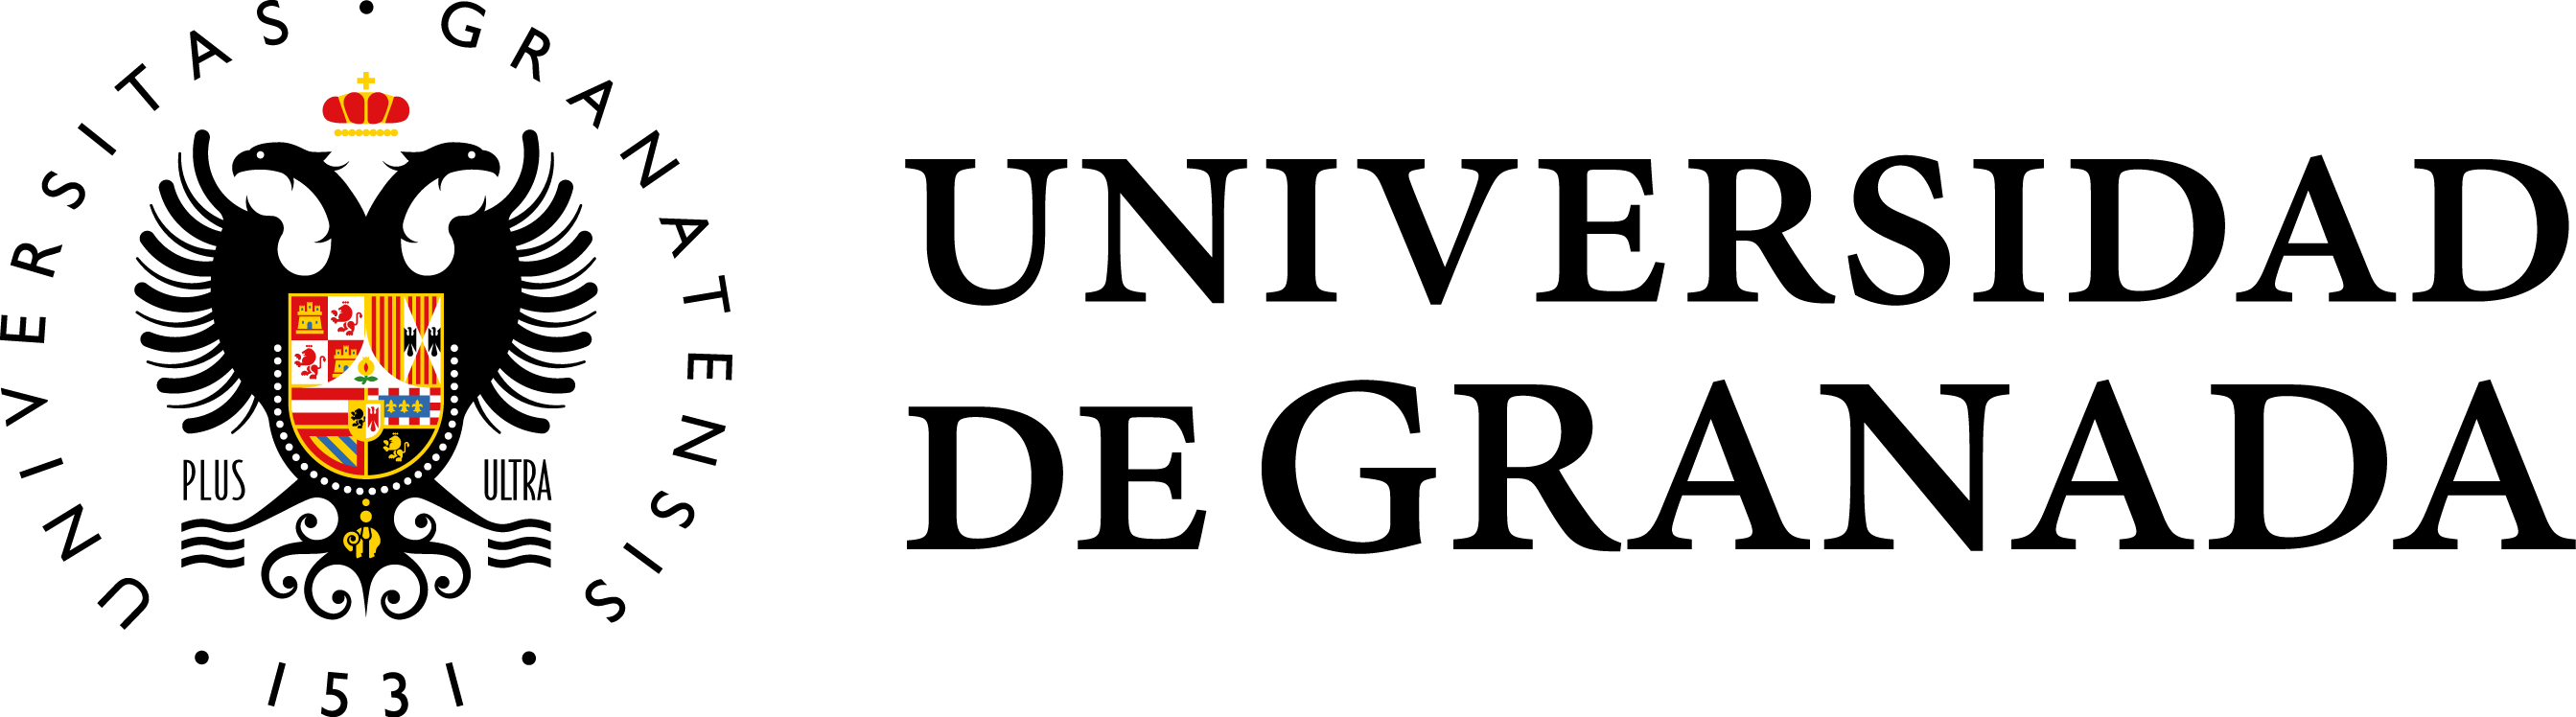
\includegraphics[width=0.25\textwidth]{../../../../extraFiles/img/ugr.png} % opcional: logo
        % \vspace{1cm}
        
        % {\large \today}
    \end{center}
    
    \restoregeometry
\end{titlepage}


%==========================
% LICENCIA
%==========================

\begin{tikzpicture}[remember picture,overlay]
\node[anchor=south west, xshift=1cm, yshift=1cm] at (current page.south west) {
\begin{minipage}{0.4\textwidth}
\begin{flushleft}
\section*{Licencia}

Este trabajo está bajo una 
\href{https://creativecommons.org/licenses/by-nc-nd/4.0/}{Licencia Creative Commons BY-NC-ND 4.0}.

\bigskip

Permisos: Se permite compartir, copiar y redistribuir el material en cualquier medio o formato.

\bigskip

Condiciones: Es necesario dar crédito adecuado, proporcionar un enlace a la licencia e indicar si se han realizado cambios. No se permite usar el material con fines comerciales ni distribuir material modificado.

\bigskip

\begin{center}
  \href{https://creativecommons.org/licenses/by-nc-nd/4.0/}{
\includegraphics[width=0.35\textwidth]{../../../../extraFiles/img/by-nc-nd.png}}
\end{center}
\end{flushleft}
\end{minipage}
};
\end{tikzpicture}

\thispagestyle{empty}
\clearpage

%==========================
% AUTOR
%==========================

% Página del autor
\begin{center}
    \vspace*{3cm} % Añadir más espacio en la parte superior
    {\Huge Modelos de
Computación}\\[2cm] % Incrementar el espacio entre líneas
    {\Large Ismael Sallami Moreno}\\[1cm] % Incrementar el espacio entre líneas
    % \includegraphics[width=0.3\textwidth]{autor.jpg} % opcional foto
    \vfill % Añadir espacio flexible para centrar verticalmente
\end{center}
\thispagestyle{empty}

% Página en blanco sin estilo
\newpage
\thispagestyle{empty}
\mbox{}

% Otra página en blanco sin estilo
\newpage
\thispagestyle{empty}
\mbox{}


%==========================
% BIOGRAFÍA
%==========================

% Breve descripción del autor
% \chapter*{Biografía}
% \addcontentsline{toc}{chapter}{Biografía} % aparece en índice
% Aquí escribes una breve descripción sobre ti, tu formación, experiencia, etc.
% \cleardoublepage


% % ===============================
% licencia.tex
% ===============================
\section*{Licencia}

Este trabajo está licenciado bajo una 
\href{https://creativecommons.org/licenses/by-nc-nd/4.0/}{Licencia Creative Commons Reconocimiento-NoComercial-SinObraDerivada 4.0 Internacional}.

\bigskip

\textbf{Usted es libre de:}
\begin{itemize}
  \item \textbf{Compartir} — copiar y redistribuir el material en cualquier medio o formato.
\end{itemize}

\bigskip

\textbf{Bajo los siguientes términos:}
\begin{description}
  \item[\textbf{Reconocimiento}] Debe otorgar el crédito adecuado, proporcionar un enlace a la licencia e indicar si se han realizado cambios. Puede hacerlo de cualquier manera razonable, pero no de una manera que sugiera que tiene el apoyo del licenciante o lo recibe por el uso que hace.

  \item[\textbf{NoComercial}] No puede utilizar el material para fines comerciales.

  \item[\textbf{SinObraDerivada}] Si remezcla, transforma o crea a partir del material, no puede distribuir el material modificado.
\end{description}

\bigskip

\begin{center}
  \href{https://creativecommons.org/licenses/by-nc-nd/4.0/}{
\includegraphics[width=0.35\textwidth]{../../../extraFiles/img/by-nc-nd.png}}
\end{center}
  % licencia
% \thispagestyle{empty} % quitar número de página en la portada
% \clearpage

% --- Índice ---
\tableofcontents
% \listoffigures
\clearpage
\thispagestyle{empty} % quitar estilo de la página en blanco

%\listoftables
%\clearpage
%\thispagestyle{empty} % quitar número de página en la portada
%\clearpage
%
% Índice de código
%\renewcommand{\lstlistlistingname}{Índice de Código}
%\lstlistoflistings
%\clearpage
%
% Índice de ecuaciones
%\renewcommand{\listtheoremname}{Índice de Ecuaciones}
%\listoftheorems[ignoreall,show={equation}]
%\clearpage

% --- Contenido Markdown generado por Pandoc ---
\part{Teoría}
\chapter{Introducción a la Computación}

\section{Fundamentos y Orígenes}

\subsection{Preguntas Clave: Definición, problemas resolubles, y Modelos de Computación}

La Ciencia de la Computación se fundamenta en la búsqueda de respuestas a preguntas trascendentales sobre los límites de la resolución automática de problemas. Entre las cuestiones centrales se encuentran:
\begin{itemize}
    \item \textbf{¿Qué puede ser resuelto de forma automática?} Esta pregunta indaga sobre la existencia de algoritmos para problemas dados, es decir, procedimientos mecánicos sistemáticos que garantizan una terminación para cualquier entrada válida.
    \item \textbf{¿Qué puede ser resuelto de forma eficiente?} Más allá de la mera resolubilidad, este interrogante aborda la viabilidad práctica de los algoritmos en términos de recursos computacionales como tiempo y espacio.
    \item \textbf{¿Qué estructuras son comunes en la computación con símbolos y cómo pueden ser procesadas?} Esta línea de investigación se enfoca en el estudio de patrones en conjuntos de cadenas y en los mecanismos formales para su manipulación.
\end{itemize}
Para abordar estas preguntas, se desarrollan \textbf{Modelos de Computación}. Estos modelos son abstracciones matemáticas de un dispositivo de cómputo, que permiten analizar sus capacidades y limitaciones de manera formal. Un concepto clave en este ámbito es el de \textbf{autómata}, concebido como un sistema algebraico que procesa información. Un autómata, en su forma más general, se define por sus conjuntos de estados, señales de entrada y señales de salida, junto con las operaciones que gobiernan sus transiciones y respuestas. El estudio de estos modelos, como las Máquinas de Turing y sus simplificaciones (autómatas finitos, autómatas con pila), constituye la base de la Teoría de la Computabilidad y de Lenguajes Formales.

\subsection{Breve Historia: Desde precursores hasta Autómatas y el Problema de la Parada}

Los fundamentos de la computación se remontan a los trabajos de lógicos y matemáticos como Russell, Hilbert y Boole, quienes sentaron las bases del formalismo matemático moderno. En las décadas de 1930 y 1940, figuras como Alan Turing y Alonzo Church formalizaron la noción de "computabilidad". Turing, en particular, propuso un modelo teórico, la \textbf{Máquina de Turing}, que se considera la definición de un dispositivo de cómputo universal.

En su búsqueda por resolver los 23 problemas propuestos por David Hilbert, la comunidad científica demostró que ciertos problemas son \textbf{indecidibles}, es decir, no admiten una solución algorítmica general. El ejemplo canónico es el \textbf{Problema de la Parada (Halting Problem)}.

\begin{definicion}[Problema de la Parada]
    No existe un programa de ordenador universal, llamémoslo \texttt{Stops(P, x)}, que pueda tomar como entrada cualquier otro programa \texttt{P} y unos datos \texttt{x} y determinar, en un tiempo finito, si \texttt{P} terminará su ejecución con la entrada \texttt{x} o si entrará en un bucle infinito.
\end{definicion}

La imposibilidad de resolver este problema fue un resultado trascendental que estableció los límites fundamentales de lo que puede ser computado.

Paralelamente, el desarrollo de los primeros lenguajes de programación como FORTRAN, COBOL y LISP en los años 50 impulsó el estudio de la sintaxis. En esta década, Noam Chomsky, junto con Michael Rabin y Dana Scott, formalizó la teoría de los \textbf{Autómatas y Lenguajes Formales}, estableciendo una jerarquía de gramáticas y máquinas que reconocen distintas clases de patrones.

\section{Elementos Básicos: Lenguajes Formales}

\subsection{Alfabetos}

La teoría de lenguajes formales se construye a partir de conceptos básicos. El más fundamental es el de alfabeto.

\begin{definicion}[Alfabeto]
Un \textbf{alfabeto} es un conjunto \textbf{finito} y no vacío de elementos denominados \textbf{símbolos} o \textbf{letras}.
\end{definicion}

\begin{anotacion}
Se denotan los alfabetos con letras mayúsculas como $\Sigma$, $A$, $B$, etc., y sus símbolos con letras minúsculas como $a, b, c$ o números.
\end{anotacion}

\begin{ejemplo}
Algunos alfabetos comunes son:
\begin{itemize}
    \item El alfabeto binario: $\Sigma = \{0, 1\}$.
    \item El alfabeto de letras minúsculas: $\Sigma = \{a, b, c, \dots, z\}$.
    \item Un alfabeto de vectores: $B = \{\langle 0,0 \rangle, \langle 0,1 \rangle, \langle 1,0 \rangle, \langle 1,1 \rangle\}$.
\end{itemize}
\end{ejemplo}

\subsection{Palabras}

\begin{definicion}[Palabra]
Una \textbf{palabra} (también llamada \textbf{cadena} o \textbf{string}) sobre un alfabeto $A$ es una sucesión finita de símbolos de $A$. La \textbf{longitud} de una palabra $u$, denotada por $|u|$, es el número de símbolos que la componen.
\end{definicion}

\begin{anotacion}
Las palabras se denotan con letras minúsculas como $u, v, w, x, y, z$. El conjunto de todas las palabras posibles sobre un alfabeto $A$ se denota como $A^*$.
\end{anotacion}

\begin{definicion}[Palabra Vacía]
La \textbf{palabra vacía}, denotada por $\epsilon$ (o a veces $\lambda$), es la única palabra de longitud cero, $| \epsilon | = 0$. Es un elemento de $A^*$ para cualquier alfabeto $A$.
\end{definicion}

\begin{anotacion}
El conjunto de todas las palabras no vacías sobre un alfabeto $A$ se denota como $A^+$. Por lo tanto, $A^+ = A^* \setminus \{\epsilon\}$.
\end{anotacion}

El conjunto de palabras $A^*$ con la operación de concatenación forma una estructura algebraica conocida como monoide, donde la palabra vacía $\epsilon$ es el elemento neutro.

\subsection{Lenguajes}

\begin{definicion}[Lenguaje]
Un \textbf{lenguaje} $L$ sobre un alfabeto $A$ es cualquier subconjunto de $A^*$, es decir, $L \subseteq A^*$. Las palabras que pertenecen al lenguaje se denominan a menudo "cadenas del lenguaje" o "frases".
\end{definicion}

\begin{ejemplo}
    Dado el alfabeto $A = \{a, b\}$:
    \begin{itemize}
        \item $L_1 = \{a, b, \epsilon\}$ es un lenguaje finito con tres palabras.
        \item $L_2 = \{a^ib^i \mid i \geq 0\}$ es un lenguaje infinito que contiene palabras con igual número de a's seguidas de b's.
        \item $L_3 = \{uu^{-1} \mid u \in \{a, b\}^*\}$ es el lenguaje de los palíndromos de longitud par.
        \item $L_4 = \{a^{n^2} \mid n \geq 1\}$ es el lenguaje de cadenas de a's cuya longitud es un cuadrado perfecto.
    \end{itemize}
\end{ejemplo}

Una propiedad fundamental del conjunto de todos los lenguajes sobre un alfabeto no vacío es su \textbf{no numerabilidad}. Mientras que el conjunto de todas las palabras $A^*$ es numerable, el conjunto de todos sus subconjuntos (es decir, el conjunto de todos los lenguajes, $\mathcal{P}(A^*)$) es no numerable. Esto tiene una profunda implicación: existen más lenguajes que programas para describirlos o reconocerlos, lo que demuestra que debe haber problemas (lenguajes) que no son computacionalmente resolubles.

\section{Operaciones Esenciales}

\subsection{Sobre Palabras}

Existen varias operaciones fundamentales que se pueden aplicar a las palabras.

\begin{definicion}[Concatenación]
Dados $u = a_1 \dots a_n$ y $v = b_1 \dots b_m$ dos palabras sobre un alfabeto $A$, su \textbf{concatenación}, denotada $uv$, es la palabra $a_1 \dots a_n b_1 \dots b_m$.
\end{definicion}
La concatenación es asociativa y tiene a $\epsilon$ como elemento neutro ($u\epsilon = \epsilon u = u$).

\begin{definicion}[Iteración]
La \textbf{iteración n-ésima} de una palabra $u$, denotada $u^n$, es la concatenación de $u$ consigo misma $n$ veces. Se define formalmente como $u^0 = \epsilon$ y $u^{i+1} = u^i u$ para $i \geq 0$.
\end{definicion}

\begin{definicion}[Palabra Inversa]
La \textbf{palabra inversa} de $u = a_1 \dots a_n$, denotada $u^{-1}$, es la palabra $a_n \dots a_1$.
\end{definicion}

\begin{anotacion}
La operación de inversión no es un homomorfismo. Por ejemplo, si $f(u) = u^{-1}$, entonces $f(uv) = (uv)^{-1} = v^{-1}u^{-1}$, que en general es distinto de $f(u)f(v) = u^{-1}v^{-1}$.
\end{anotacion}

\subsection{Sobre Lenguajes}

Al ser los lenguajes conjuntos de palabras, heredan las operaciones de conjuntos como la \textbf{unión} ($L_1 \cup L_2$), \textbf{intersección} ($L_1 \cap L_2$) y \textbf{complementario} ($\bar{L} = A^* \setminus L$). Adicionalmente, se definen operaciones específicas.

\begin{definicion}[Concatenación de Lenguajes]
La \textbf{concatenación} de dos lenguajes $L_1$ y $L_2$ es el lenguaje $L_1 L_2 = \{uv \mid u \in L_1, v \in L_2\}$.
\end{definicion}
Esta operación es asociativa y tiene como elemento neutro el lenguaje $\{\epsilon\}$.

\begin{definicion}[Clausura de Kleene y Clausura Positiva]
Dado un lenguaje $L$, su \textbf{clausura de Kleene} (o estrella), denotada $L^*$, es la unión de todas sus potencias:
\[ L^* = \bigcup_{i \geq 0} L^i = L^0 \cup L^1 \cup L^2 \cup \dots \]
La \textbf{clausura positiva}, denotada $L^+$, se define de manera similar pero excluyendo la potencia cero:
\[ L^+ = \bigcup_{i \geq 1} L^i = L^1 \cup L^2 \cup \dots \]
donde $L^0 = \{\epsilon\}$ y $L^{i+1} = L L^i$.
\end{definicion}
Se cumple que $L^+ = L^*$ si y solo si $\epsilon \in L$. Si $\epsilon \notin L$, entonces $L^* = L^+ \cup \{\epsilon\}$. Si $L$ es un lenguaje no vacío, $L^*$ siempre es infinito.

\section{Generación de Lenguajes}

\subsection{Gramáticas: Definición y Lenguaje Generado}
Los lenguajes, especialmente los infinitos, requieren un mecanismo finito para su descripción. Las gramáticas generativas, introducidas por Noam Chomsky, son uno de dichos mecanismos.

\begin{definicion}[Gramática Generativa]
Una \textbf{gramática generativa} es una tupla $G = (V, T, P, S)$, donde:
\begin{itemize}
    \item $V$ es un alfabeto finito de \textbf{variables} o símbolos no terminales.
    \item $T$ es un alfabeto finito de \textbf{símbolos terminales}, disjunto de $V$.
    \item $P$ es un conjunto finito de \textbf{reglas de producción} de la forma $\alpha \rightarrow \beta$, donde $\alpha, \beta \in (V \cup T)^*$ y $\alpha$ contiene al menos una variable.
    \item $S \in V$ es el \textbf{símbolo inicial} o axioma.
\end{itemize}
\end{definicion}

Una palabra $\beta$ se \textbf{deriva} de $\alpha$ en un paso ($\alpha \Rightarrow \beta$) si existe una regla $\gamma \rightarrow \phi \in P$ y $\alpha$ puede escribirse como $\alpha_1\gamma\alpha_2$, de tal forma que $\beta = \alpha_1\phi\alpha_2$. La relación de derivación en múltiples pasos se denota por $\Rightarrow^*$.

\begin{definicion}[Lenguaje Generado]
El \textbf{lenguaje generado} por una gramática $G$, denotado $L(G)$, es el conjunto de todas las palabras compuestas exclusivamente por símbolos terminales que pueden derivarse a partir del símbolo inicial $S$:
\[ L(G) = \{ u \in T^* \mid S \Rightarrow^* u \} \].
\end{definicion}

\begin{ejemplo}
Sea la gramática $G = (\{S\}, \{a, b\}, \{S \rightarrow aSb, S \rightarrow \epsilon\}, S)$.
Esta gramática genera el lenguaje $L(G) = \{a^i b^i \mid i \geq 0\}$. Por ejemplo, para generar $aabb$:
$S \Rightarrow aSb \Rightarrow aaSbb \Rightarrow aab\epsilon b = aabb$.
\end{ejemplo}

\subsection{Jerarquía de Chomsky}

Noam Chomsky clasificó las gramáticas en cuatro tipos, estableciendo una jerarquía basada en las restricciones impuestas sobre sus reglas de producción.

\begin{definicion}[Jerarquía de Chomsky]
La jerarquía de Chomsky se define de la siguiente manera:
\begin{itemize}
    \item \textbf{Tipo 0 (Sin restricciones):} Corresponde a cualquier gramática generativa. Estas gramáticas generan los lenguajes \textbf{recursivamente enumerables}, que son aquellos reconocibles por una Máquina de Turing.
    \item \textbf{Tipo 1 (Dependientes del contexto):} Todas las producciones son de la forma $\alpha_1 A \alpha_2 \rightarrow \alpha_1 \beta \alpha_2$, con $A \in V$, $\alpha_1, \alpha_2, \beta \in (V \cup T)^*$ y $\beta \neq \epsilon$. Se permite la regla $S \rightarrow \epsilon$ si $S$ no aparece en la parte derecha de ninguna regla. Generan los lenguajes \textbf{dependientes del contexto}. Un ejemplo es el lenguaje $\{a^n b^n c^n \mid n \geq 1\}$.
    \item \textbf{Tipo 2 (Independientes del contexto):} Todas las producciones son de la forma $A \rightarrow \alpha$, con $A \in V$ y $\alpha \in (V \cup T)^*$. Generan los lenguajes \textbf{independientes del contexto}.
    \item \textbf{Tipo 3 (Regulares):} Todas las producciones son de la forma $A \rightarrow uB$ o $A \rightarrow u$, donde $A, B \in V$ y $u \in T^*$. Generan los \textbf{lenguajes regulares}.
\end{itemize}
\end{definicion}

Esta jerarquía establece una relación de inclusión estricta entre las familias de lenguajes generados, denotadas por $\mathcal{L}_i$ para el tipo $i$:
\[ \mathcal{L}_3 \subset \mathcal{L}_2 \subset \mathcal{L}_1 \subset \mathcal{L}_0 \].
Por ejemplo, todo lenguaje regular es también independiente del contexto, pero no a la inversa.
\chapter{Autómatas Finitos y Lenguajes Regulares}

\section{Fundamentos y Aplicaciones de los Autómatas Finitos}

\subsection{Contexto y Relevancia}

\subsubsection{Importancia de los Autómatas Finitos (AF) en la computación}

Los Autómatas Finitos (AF) constituyen modelos matemáticos esenciales que residen en el núcleo teórico de la Ciencia de la Computación. El estudio de los autómatas es fundamental para investigar qué puede resolverse de forma automática y qué estructuras, basadas en palabras y símbolos, pueden procesarse eficientemente en un ordenador. El concepto de autómata surge en diversos problemas asociados con la informática, los sistemas de redes y la teoría de control. La estructura matemática de los autómatas se basa en argumentos intuitivos que reflejan la entidad de los autómatas reales (no necesariamente físicos).

\begin{itemize}
    \item \text{Aplicaciones en análisis léxico (compiladores):}
    Una aplicación práctica crucial de los AF se encuentra en la \text{construcción de analizadores léxicos} (lexers) dentro de los compiladores. Un analizador léxico tiene la función de reconocer secuencias de caracteres que forman \textit{tokens} (como palabras clave o identificadores), un problema que se mapea directamente al reconocimiento de \text{lenguajes regulares}.

    \item \text{Verificación de circuitos digitales:}
    Los AF son ampliamente utilizados en el desarrollo de software destinado al \text{diseño y la verificación de circuitos digitales}. Esto es pertinente porque los autómatas modelan sistemas que operan en un número finito de estados diferentes.

    \item \text{Análisis de patrones de texto (ej. correos electrónicos):}
    Los autómatas finitos se emplean extensamente en software para \text{analizar grandes volúmenes de texto} en busca de patrones específicos, tales como palabras, estructuras o formatos predefinidos (por ejemplo, en páginas web o para encontrar direcciones de correo electrónico). También son útiles para comprobar la corrección de cualquier sistema que posea un número finito de estados distintos, como los protocolos de comunicación.
\end{itemize}

\begin{anotacion}{El Marco Algebraico de los Autómatas.}
La investigación de las \text{estructuras algebraicas} sugeridas por el concepto de autómata permite desarrollar una teoría profunda. Estos modelos, incluidos los autómatas y las bases de datos, se manifiestan como \text{estructuras algebraicas de múltiples tipos} (\textit{many-sorted algebraic structures}). El tratamiento de estas estructuras permite estudiar el comportamiento y la estructura de los autómatas reales.
\end{anotacion}

\subsection{Nociones Preliminares}

Para comprender un autómata, se requiere un entendimiento previo de los lenguajes formales. Un \text{lenguaje} $L$ sobre un alfabeto $A$ se define formalmente como un \text{subconjunto} del conjunto de todas las cadenas posibles sobre $A$, denotado como $A^*$. El autómata tiene la función de aceptar las palabras $u \in A^*$ que pertenecen a $L$.

\subsubsection{Ejemplo introductorio mediante un diagrama de transición}

Un Autómata Finito Determinista (AFD) $M = (Q, A, \delta, q_0, F)$ se define a través de un conjunto de estados ($Q$), un alfabeto de entrada ($A$), una función de transición ($\delta$), un estado inicial ($q_0$) y un conjunto de estados finales ($F$). Un \text{diagrama de transición} proporciona una representación visual e intuitiva de esta estructura.

Consideremos un AFD $M$ sobre el alfabeto $A=\{0, 1\}$ cuyo lenguaje aceptado, $L(M)$, consiste en todas las palabras que \text{contienen la subcadena $\mathbf{00}$}.

\begin{ejemplo}[AFD: Reconocimiento de Subcadena 00]
El autómata se construye con tres estados: $q_0$ (inicial), $q_1$ (se leyó un '0'), y $q_2$ (se leyó '00' y es final). 

\begin{figure}[H]
    \centering
    \begin{tikzpicture}[>={Stealth[round]}, node distance=2.5cm, auto, shorten >=1pt] % Configuración basada en

        % Estados
        \node[state, initial] (q0) {$q_0$}; % Estado inicial
        \node[state, right of=q0] (q1) {$q_1$};
        \node[state, accepting, right of=q1] (q2) {$q_2$};
        
        % Transiciones
        % q0: No ha leído un '0' o ha leído '1'
        \draw[->] (q0) edge[loop above] node {1} (q0);
        \draw[->] (q0) -- (q1) node[midway, above] {0};
        
        % q1: Acaba de leer '0'. Espera otro '0'
        \draw[->] (q1) edge[bend left] node {1} (q0);
        \draw[->] (q1) -- (q2) node[midway, above] {0};
        
        % q2: Ha leído '00'. Estado final (sumidero de aceptación)
        \draw[->] (q2) edge[loop above] node {0, 1} (q2);
        
    \end{tikzpicture}
    \captionof{figure}{Autómata Finito Determinista que acepta el lenguaje de palabras que contienen la subcadena 00.}
    \label{fig:afd_00}
\end{figure}

\text{Proceso de Cálculo:} La aceptación de una palabra $u$ se define a través de una \text{relación de cálculo} $(C_i \vdash C_{i+1})$, donde $C_i = (q, v)$ es una configuración (estado $q$, cadena restante $v$).

\begin{itemize}
    \item \text{Aceptación de \codeinline{100}:} El autómata comienza en $(q_0, 100)$ y termina en un estado final $q_2$ con la cadena vacía $\varepsilon$:
    \[ (q_0, 100) \vdash (q_0, 00) \vdash (q_1, 0) \vdash (q_2, \varepsilon) \]
    Dado que $q_2$ es un estado final, \codeinline{100} es aceptada.

    \item \text{Rechazo de \codeinline{101}:} El proceso termina en $q_0$, que no es un estado final, resultando en el rechazo:
    \[ (q_0, 101) \vdash (q_0, 01) \vdash (q_1, 1) \vdash (q_0, \varepsilon) \]
\end{itemize}

El lenguaje aceptado $L(M)$ es el conjunto de todas las palabras $u \in A^*$ tales que, partiendo del estado inicial $q_0$ y consumiendo $u$, el autómata finaliza en algún estado $q \in F$. Para este ejemplo, $L(M) = \{u_1 00 u_2 \in \{0, 1\}^* \mid u_1, u_2 \in \{0, 1\}^*\}$.
\end{ejemplo}







\section{Autómata Finito Determinista (AFD)} % Corresponde a Índice 2.

\subsection{Definición Formal} % Corresponde a Índice 2.1.
El Autómata Finito Determinista (AFD) sirve como el modelo fundamental más sencillo para estudiar la computabilidad y los lenguajes regulares. Su naturaleza determinista radica en que, dado un estado y un símbolo de entrada, el estado siguiente está unívocamente definido.

\subsubsection{La quíntupla $M=(Q,A,\delta,q_0,F)$}
Un AFD se define formalmente como una quíntupla:
\[ M = (Q, A, \delta, q_0, F) \]
donde cada componente juega un papel crucial en la definición de la máquina de estados:
\begin{itemize}
    \item $Q$: Es el \text{conjunto finito} de estados del autómata.
    \item $A$: Es el \text{alfabeto} o conjunto de entrada, que debe ser un conjunto finito de símbolos o letras.
    \item $\delta$: Es la \text{función de transición}. Para un AFD, esta es una aplicación $\delta : Q \times A \to Q$. La función $\delta$ especifica la transición de un estado a otro de manera única para cada par (estado, símbolo).
    \item $q_0$: Es el \text{estado inicial}, un elemento distinguido $q_0 \in Q$.
    \item $F$: Es el \text{conjunto de estados finales} o de aceptación, siendo un subconjunto de $Q$, $F \subseteq Q$.
\end{itemize}

\subsection{Representación} % Corresponde a Índice 2.2.

Los AFD pueden representarse de diferentes maneras, lo que facilita su análisis y comprensión, incluyendo la forma analítica, las tablas o los gráficos (\textit{plots}).

\subsubsection{Diagramas de Transición}
Los diagramas de transición (o gráficos de estados) son la forma más intuitiva de representar un autómata. En esta representación, los estados se dibujan como círculos, las transiciones $\delta(q, a) = p$ como flechas dirigidas desde $q$ a $p$ etiquetadas con $a$, el estado inicial se marca con una flecha entrante no etiquetada, y los estados finales se denotan con un doble círculo.

\begin{ejemplo}[Diagrama de Transición (AFD para subcadena 00)]
Utilizamos la representación de AFD para el lenguaje $L$ de palabras que contienen la subcadena $00$.
\begin{figure}[H]
    \centering
    \begin{tikzpicture}[>={Stealth[round]}, node distance=2.5cm, auto, shorten >=1pt]
        \node[state, initial] (q0) {$q_0$};
        \node[state, right of=q0] (q1) {$q_1$};
        \node[state, accepting, right of=q1] (q2) {$q_2$};
        \draw[->] (q0) edge[loop above] node {1} (q0);
        \draw[->] (q0) -- (q1) node[midway, above] {0};
        \draw[->] (q1) edge[bend left] node {1} (q0);
        \draw[->] (q1) -- (q2) node[midway, above] {0};
        \draw[->] (q2) edge[loop above] node {0, 1} (q2);
    \end{tikzpicture}
    \captionof{figure}{Diagrama de Transición para el AFD que acepta $00$.}
    \label{fig:afd_diagrama_ch2}
\end{figure}
\end{ejemplo}
\subsubsection{Tablas de Transición}
Las tablas de transición son una representación tabular y analítica de la función $\delta$, especialmente útil para la implementación algorítmica y la conversión entre tipos de autómatas.
\begin{ejemplo}[Tabla de Transición]
La tabla para el AFD de la Figura \ref{fig:afd_diagrama_ch2} es:
\begin{table}[H]
\centering
\begin{tabular}{|c|c|c|}
\toprule
\text{Estado} & \text{0} & \text{1} \\
\midrule
$\to q_0$ & $q_1$ & $q_0$ \\
$q_1$ & $q_2$ & $q_0$ \\
$\star q_2$ & $q_2$ & $q_2$ \\
\bottomrule
\end{tabular}
\caption{Tabla de transición del AFD para el lenguaje que contiene $00$.}
\end{table}
\end{ejemplo}

\subsection{Proceso de Cálculo} % Corresponde a Índice 2.3.

El \text{proceso de cálculo} de un AFD describe cómo evoluciona la máquina al procesar una palabra de entrada.

\subsubsection{Configuración o Descripción Instantánea} % Corresponde a Índice 2.3.1.
Una \text{configuración} o \text{descripción instantánea} se define como un par $(q, u) \in Q \times A^*$. Representa el estado actual del cómputo, donde $q$ es el estado en el que se encuentra el autómata y $u$ es la porción restante de la palabra de entrada. La configuración inicial para una palabra $u$ es siempre $(q_0, u)$.

\subsubsection{Relación de un paso de cálculo ($\vdash$) y de cálculo extendida ($\vdash^*$)} % Corresponde a Índice 2.3.2.
La \text{relación de un paso de cálculo} ($\vdash$) describe una única transición en el autómata:
\[ (q, au) \vdash (p, u) \iff \delta(q, a) = p \]
donde $q, p \in Q$, $a \in A$ (símbolo leído), y $u \in A^*$ (cadena restante). Dado que el AFD es determinista, de una configuración se puede pasar a un máximo de una configuración en un solo paso de cálculo.

La \text{relación de cálculo extendida} ($\vdash^*$) denota una secuencia finita de cero o más pasos de cálculo. La existencia de una sucesión de configuraciones $C_0, \dots, C_n$ tal que $C_0 \vdash C_1 \vdash \dots \vdash C_n$ se denota como $(q, u) \vdash^* (p, v)$.

\subsubsection{Función de Transición Extendida ($\delta^*$)} % Corresponde a Índice 2.3.3.
Para simplificar la notación de trayectorias, se define la \text{función de transición extendida} $\delta^*: Q \times A^* \to Q$. Esta función devuelve el estado final al que se llega después de leer una palabra completa $u$, partiendo de un estado $q$.

\begin{definicion}[Función de Transición Extendida $\delta^*$]
La función $\delta^*$ se define recursivamente como:
\begin{enumerate}
    \item \text{Base:} $\delta^*(q, \varepsilon) = q$, para $q \in Q$.
    \item \text{Recursión:} $\delta^*(q, au) = \delta^*(\delta(q, a), u)$, para $q \in Q$, $a \in A$, $u \in A^*$.
\end{enumerate}
\end{definicion}

\subsection{Aceptación de Palabras} % Corresponde a Índice 2.4.

La capacidad de un AFD de reconocer un patrón o estructura se define mediante el lenguaje que acepta.

\subsubsection{Definición de Lenguaje Aceptado $L(M)$ por un AFD}
Una palabra $u \in A^*$ es \text{aceptada} si el autómata, comenzando en el estado inicial $q_0$ y consumiendo toda la palabra, finaliza en un estado de aceptación $q \in F$. El conjunto de todas estas palabras aceptadas constituye el lenguaje $L(M)$.

El lenguaje $L(M)$ puede expresarse formalmente de dos formas equivalentes:

\begin{enumerate}
    \item \text{Usando la relación de cálculo extendida:}
    \[ L(M) = \{u \in A^* \mid \exists q \in F \text{ tal que } (q_0, u) \vdash^* (q, \varepsilon)\} \]
    \item \text{Usando la función de transición extendida:}
    \[ L(M) = \{u \in A^* \mid \delta^*(q_0, u) \in F\} \]
    Esta segunda expresión es inmediata y se utiliza frecuentemente en la teoría.
\end{enumerate}

\begin{ejemplo}[Aplicación de $\delta^*$]
Si consideramos el AFD del ejemplo anterior (AFD para subcadena $00$), el cálculo de $\delta^*$ para la palabra \codeinline{modern}{100} es:
\[ \delta^*(q_0, 100) = \delta^*(\delta(q_0, 1), 00) = \delta^*(q_0, 00) = \delta^*(\delta(q_0, 0), 0) = \delta^*(q_1, 0) = q_2 \]
Como $\delta^*(q_0, 100) = q_2$ y $q_2 \in F$, la palabra es aceptada.
\end{ejemplo}

\begin{anotacion}{Propiedad de Clausura.}
Todos los lenguajes que son aceptados por un AFD son también aceptados por un Autómata Finito No Determinista (AFND), ya que todo AFD se considera un caso especial de AFND.
\end{anotacion}



\section{Tipos de Autómatas Finitos y Equivalencias} % Corresponde a Índice 3.

El estudio de los Autómatas Finitos (AF) requiere examinar extensiones del modelo determinista que facilitan la modelización y la composición. Los AFND y los AFN-$\epsilon$ son formalmente más potentes en su expresividad, aunque se demuestra que no reconocen una clase de lenguajes mayor que los AFD.

\subsection{Autómata Finito No Determinista (AFND)} % Corresponde a Índice 3.1.

Mientras que un Autómata Finito Determinista (AFD) tiene una única transición definida para cada par (estado, símbolo), el Autómata Finito No Determinista (AFND) introduce la posibilidad de que, dada una entrada, la máquina pueda evolucionar a múltiples estados siguientes o a ninguno.

\subsubsection{Definición formal con función de transición a conjuntos de estados: $\delta: Q \times A \to \mathcal{P}(Q)$}

Un AFND se define formalmente como una quíntupla $M = (Q, A, \delta, q_0, F)$, similar al AFD, pero con una diferencia crítica en su función de transición.

\begin{definicion}[Autómata Finito No Determinista (AFND)]
Un AFND es una quíntupla $M = (Q, A, \delta, q_0, F)$, donde:
\begin{itemize}
    \item $Q$ es el conjunto finito de estados.
    \item $A$ es el alfabeto de entrada.
    \item $\delta$ es la \text{función de transición} que mapea un par (estado, símbolo) a un \text{conjunto de estados}:
    \[ \delta : Q \times A \to \mathcal{P}(Q) \]
    donde $\mathcal{P}(Q)$ es el conjunto potencia de $Q$ (todos los subconjuntos de $Q$).
    \item $q_0 \in Q$ es el estado inicial.
    \item $F \subseteq Q$ es el conjunto de estados finales.
\end{itemize}
\end{definicion}

El no determinismo implica que la \text{relación de cálculo} $((q, au) \vdash (p, u))$ se cumple si $p \in \delta(q, a)$, permitiendo que haya múltiples caminos de cómputo para una misma palabra de entrada, o incluso ninguno. Una palabra es aceptada si \text{existe al menos un camino de cálculo} que consume toda la palabra y termina en un estado de aceptación.

\begin{ejemplo}[AFND con Múltiples Transiciones]
Sea un AFND $M$ sobre $A=\{0, 1\}$ que acepta palabras que contienen la subcadena \codeinline{001}. Observamos que desde $q_0$, al leer \codeinline{0}, la transición no es única:
\begin{figure}[H]
    \centering
    \begin{tikzpicture}[>={Stealth[round]}, node distance=2.5cm, auto, shorten >=1pt]
        % Estados
        \node[state, initial] (q0) {$q_0$};
        \node[state, right of=q0] (q1) {$q_1$};
        \node[state, right of=q1] (q2) {$q_2$};
        \node[state, accepting, right of=q2] (q3) {$q_3$};
        
        % Transiciones
        % Bucle para 0, 1 en q0 (permitiendo comenzar 001 en cualquier momento)
        \draw[->] (q0) edge[loop above] node {0, 1} (q0);
        
        % Transición no determinista que inicia la subcadena
        \draw[->] (q0) edge[bend left] node {0} (q1);
        
        % Camino de aceptación 001
        \draw[->] (q1) -- (q2) node[midway, above] {0};
        \draw[->] (q2) -- (q3) node[midway, above] {1};
        
        % Bucle para 0, 1 en q3
        \draw[->] (q3) edge[loop above] node {0, 1} (q3);
        
    \end{tikzpicture}
    \captionof{figure}{AFND para el lenguaje que contiene la subcadena 001. Desde $q_0$ con el símbolo 0 se puede ir a $q_0$ o a $q_1$, ilustrando la no determinismo.}
\end{figure}
\end{ejemplo}

\subsection{AFND con Transiciones Nulas (AFN-$\epsilon$)} % Corresponde a Índice 3.2.

Los AFND se extienden aún más al permitir movimientos entre estados que no consumen ningún símbolo de la cadena de entrada. Estos son los AFND con transiciones nulas o \textit{épsilon} (AFN-$\epsilon$).

\subsubsection{Inclusión del símbolo de palabra vacía ($\epsilon$) en el alfabeto para las transiciones}

Un AFN-$\epsilon$ es una quíntupla $M = (Q, A, \delta, q_0, F)$ donde la función de transición $\delta$ incluye la palabra vacía $\epsilon$ en su dominio:
\[ \delta : Q \times (A \cup \{\epsilon\}) \to \mathcal{P}(Q) \]

Las transiciones $\epsilon$ permiten que la descripción instantánea cambie de estado sin avanzar la posición de lectura en la cadena de entrada. Esto resulta extremadamente útil para construir autómatas que simulan operaciones de lenguajes formales, como la unión ($r_1 + r_2$) o la clausura de Kleene ($r_1^*$), ya que se pueden conectar sub-autómatas utilizando estas transiciones sin afectar la semántica del lenguaje reconocido.

\begin{ejemplo}[Utilidad de $\epsilon$ en la Unión]
Para modelar la unión de dos lenguajes, $L_1$ y $L_2$, se puede crear un nuevo estado inicial $q_0$ y añadir transiciones $\epsilon$ a los estados iniciales de los autómatas de $L_1$ y $L_2$.
\end{ejemplo}

\subsection{Conversión AFND $\to$ AFD} % Corresponde a Índice 3.3.

A pesar de la mayor complejidad operativa de los AFND, la clase de lenguajes que aceptan es exactamente la misma que la de los AFD. Esta equivalencia se establece mediante un algoritmo constructivo.

\subsubsection{Presentación del Método de los Subconjuntos como algoritmo de equivalencia}

El algoritmo para convertir un AFND $M$ en un AFD equivalente $M'$ se basa en la idea de que cada \text{estado} en el AFD $M'$ representa un \text{conjunto de posibles estados} en los que el AFND $M$ podría encontrarse después de leer un prefijo de la entrada. Este procedimiento se conoce como el \text{Método de los Subconjuntos}.

Si $M = (Q, A, \delta_N, q_0, F_N)$ es el AFND, el AFD equivalente resultante es $M' = (Q', A, \delta_D, q'_0, F_D)$, donde:
\begin{itemize}
    \item $Q'$ es un subconjunto de $\mathcal{P}(Q)$. Los estados de $M'$ son subconjuntos de estados de $M$.
    \item El estado inicial $q'_0 = \{q_0\}$ (o $\text{Cl}(q_0)$ si hubiera $\epsilon$-transiciones).
    \item Un estado $P \in Q'$ es final en $M'$ ($P \in F_D$) si y solo si contiene al menos un estado final del AFND, es decir, $P \cap F_N \neq \emptyset$.
    \item La función de transición determinista $\delta_D$ se define de la siguiente manera, para un estado $P \subseteq Q$ y un símbolo $a \in A$:
    \[ \delta_D(P, a) = \bigcup_{q \in P} \delta_N(q, a) \]
\end{itemize}
El AFD $M'$ se construye explorando progresivamente los nuevos conjuntos de estados alcanzables a partir de $q'_0$.

\subsection{Conversión AFN-$\epsilon$ $\to$ AFND} % Corresponde a Índice 3.4.

La eliminación de las transiciones $\epsilon$ es un paso crucial en la práctica, ya que simplifica el autómata y permite, en última instancia, la conversión al modelo AFD (a menudo, la conversión de AFN-$\epsilon$ a AFD se realiza en un solo paso, combinando este proceso con el método de los subconjuntos).

\subsubsection{Cálculo de la $\epsilon$-Clausura para la eliminación de transiciones nulas}

Para eliminar las transiciones $\epsilon$, se debe definir la \text{$\epsilon$-Clausura} ($\text{Cl}$), que captura todos los estados alcanzables desde un estado dado utilizando únicamente transiciones nulas.

\begin{definicion}[$\epsilon$-Clausura]
Dado un AFN-$\epsilon$ $M = (Q, A, \delta, q_0, F)$:
\begin{itemize}
    \item La \text{$\epsilon$-Clausura de un estado $q$}, denotada $\text{Cl}(q)$, es el conjunto de todos los estados $p$ tales que existe un camino de cero o más pasos de $\epsilon$-transición desde $q$ hasta $p$.
    \item La \text{$\epsilon$-Clausura de un conjunto de estados $P \subseteq Q$}, denotada $\text{Cl}(P)$, es la unión de las $\epsilon$-Clausuras de todos los estados en $P$:
    \[ \text{Cl}(P) = \bigcup_{q \in P} \text{Cl}(q) \]
\end{itemize}
\end{definicion}

La $\epsilon$-Clausura es esencial para definir la función de transición del autómata resultante $M'$ (que será un AFND sin $\epsilon$-transiciones o un AFD). La nueva función de transición, $\delta'$, se calcula utilizando la $\epsilon$-Clausura en cada paso de lectura, asegurando que se contabilicen todos los movimientos nulos previos y posteriores a la lectura del símbolo.

Formalmente, si $P$ es un conjunto de estados del AFN-$\epsilon$, la transición a partir de un símbolo $a$ en el autómata equivalente se calcula mediante la función $\delta^*$ extendida:
\[ \delta^*(P, a) = \text{Cl}\left( \bigcup_{q \in P} \delta(q, a) \right) \]
Esta $\delta^*$ (aplicada al AFN-$\epsilon$) proporciona directamente el conjunto de estados en el AFD equivalente $M'$.

\begin{anotacion}{Teorema de Equivalencia.}
La existencia de conversiones algorítmicas entre los tres modelos (AFD $\leftrightarrow$ AFND $\leftrightarrow$ AFN-$\epsilon$) demuestra que \text{todos aceptan exactamente la misma clase de lenguajes}, conocida como la clase de \text{Lenguajes Regulares}. Esto es un resultado fundamental en la teoría de la computación.
\end{anotacion}


\section{Expresiones Regulares (ER) y El Teorema de Kleene} % Corresponde a Índice 4.

La clase de los lenguajes aceptados por Autómatas Finitos (AFD, AFND, AFN-$\epsilon$) se denomina Lenguajes Regulares ($\mathcal{L}_3$). Una caracterización fundamental de esta clase es su representación mediante Expresiones Regulares (ER). La equivalencia entre estas dos notaciones constituye el célebre \text{Teorema de Kleene}.

\subsection{Concepto y Operadores} % Corresponde a Índice 4.1.

\subsubsection{Definición de Expresión Regular}

Una Expresión Regular sobre un alfabeto $A$ es una cadena de caracteres que describe un conjunto (lenguaje) de palabras mediante una definición recursiva.

\begin{definicion}[Expresión Regular (ER)]
Sea $A$ un alfabeto. Una Expresión Regular $r$ sobre $A$ es definida recursivamente como:
\begin{enumerate}
    \item La expresión $\mathbf{\emptyset}$ (o $\mathbf{/0}$) es una ER que denota el lenguaje vacío, $L(\mathbf{\emptyset}) = \emptyset$.
    \item La expresión $\mathbf{\epsilon}$ es una ER que denota el lenguaje que contiene únicamente la palabra vacía, $L(\mathbf{\epsilon}) = \{\varepsilon\}$.
    \item Para cada símbolo $a \in A$, la expresión $\mathbf{a}$ es una ER que denota el lenguaje que contiene únicamente la palabra $a$, $L(\mathbf{a}) = \{a\}$.
    \item Si $r_1$ y $r_2$ son ERs, entonces la \text{Unión} $(r_1 + r_2)$, la \text{Concatenación} $(r_1 r_2)$ y la \text{Clausura de Kleene} $(r_1^*)$ son también ERs.
\end{enumerate}
\end{definicion}

\subsubsection{Operaciones fundamentales}

Los operadores de las ERs corresponden directamente a operaciones sobre los lenguajes formales:

\begin{itemize}
    \item \text{Unión (o suma) ($+$):}
    Si $L_1 = L(r_1)$ y $L_2 = L(r_2)$, la unión de $r_1$ y $r_2$, denotada $r_1 + r_2$, representa la unión de los lenguajes: $L(r_1 + r_2) = L_1 \cup L_2$. Es conmutativa y asociativa.

    \item \text{Concatenación (yuxtaposición):}
    La concatenación $r_1 r_2$ denota el conjunto de palabras formadas al concatenar cualquier palabra de $L_1$ con cualquier palabra de $L_2$: $L(r_1 r_2) = \{uv \mid u \in L_1, v \in L_2\}$. La concatenación es asociativa y $\epsilon$ es su elemento neutro ($r\epsilon = r$).

    \item \text{Clausura de Kleene ($\mathbf{*}$):}
    La clausura de Kleene de una expresión $r$, denotada $r^*$, representa la \text{iteración} del lenguaje asociado $L(r)$.
    \[ L(r)^* = \bigcup_{i \geq 0} L(r)^i \]
    donde $L(r)^0 = \{\varepsilon\}$. Esta operación garantiza la aceptación de cero o más repeticiones de patrones definidos por $r$.
\end{itemize}

\begin{ejemplo}[Expresiones Regulares]
Sea $A=\{0, 1\}$.
\begin{enumerate}
    \item La expresión \codeinline{(0+1)*} denota todas las palabras posibles sobre $A$, $A^*$.
    \item La expresión \codeinline{1*(01*01*)*1*} denota el lenguaje de palabras donde el número de ceros es par, incluyendo la palabra vacía y palabras compuestas únicamente de unos. (Nota: La versión simplificada en la fuente es \codeinline{1*(01*01*)*}, que acepta palabras que inician con 1s y tienen un número par de 0s, con 1s intercalados, y debe cerrarse con $1^*$ o ser ajustada para la definición completa del lenguaje).
    \item La expresión \codeinline{(0+1)*0110(0+1)*} denota el lenguaje de palabras que contienen la subcadena \codeinline{0110}.
\end{enumerate}
\end{ejemplo}

\subsection{Conversión Autómata Finito $\to$ Expresión Regular (Teorema de Kleene, Parte I)} % Corresponde a Índice 4.2.

La primera parte del Teorema de Kleene afirma que, si un lenguaje $L$ es aceptado por un Autómata Finito Determinista (AFD), entonces $L$ puede ser expresado mediante una Expresión Regular. El método constructivo para obtener la ER asociada a un AFD $M=(Q, A, \delta, q_1, F)$ se basa en la \text{eliminación de estados} de forma recursiva.

Asumimos que los estados de $M$ están numerados $Q = \{q_1, q_2, \ldots, q_n\}$.

\subsubsection{Definición del conjunto $R_{ij}^k$} % Corresponde a Índice 4.2.1.

El cálculo se articula alrededor de la definición de los conjuntos $R_{ij}^k$, donde $k$ representa un límite superior para los índices de los estados intermedios permitidos en un camino.

\begin{definicion}[Conjunto de Palabras $R_{ij}^k$]
$R_{ij}^k$ es el conjunto de todas las palabras $u \in A^*$ tales que, si el autómata comienza en el estado $q_i$ y finaliza en el estado $q_j$ después de leer $u$, todos los estados intermedios por los que pasa el autómata (al leer cualquier prefijo propio de $u$) tienen un índice (numeración) \text{menor o igual a $k$}.
\end{definicion}

El valor de $k$ varía desde $0$ hasta $n$, donde $n = |Q|$.

\subsubsection{Algoritmo recursivo y fórmula de cálculo} % Corresponde a Índice 4.2.2.

Para calcular $R_{ij}^k$, se divide el conjunto de caminos de $q_i$ a $q_j$ (con estados intermedios $\le k$) en dos categorías:

\begin{enumerate}
    \item Caminos que \text{no pasan} por el estado $q_k$. Estos caminos ya estaban incluidos en $R_{ij}^{k-1}$.
    \item Caminos que pasan por $q_k$ \text{una o más veces}.
\end{enumerate}

Los caminos del tipo 2 se descomponen en cuatro partes, usando el estado $q_k$ como punto de bifurcación:
\begin{enumerate}
    \item Un camino de $q_i$ a $q_k$ que solo usa estados intermedios $\le k-1$ ($R_{ik}^{k-1}$).
    \item Cero o más bucles en $q_k$ (de $q_k$ a $q_k$) que solo usan estados intermedios $\le k-1$ ($R_{kk}^{k-1})^*$.
    \item Un camino final de $q_k$ a $q_j$ que solo usa estados intermedios $\le k-1$ ($R_{kj}^{k-1}$).
\end{enumerate}

La fórmula de recurrencia para el conjunto $R_{ij}^k$ es:
\[ R_{ij}^k = R_{ij}^{k-1} \cup R_{ik}^{k-1} (R_{kk}^{k-1})^* R_{kj}^{k-1} \]
De esta definición se deriva directamente la fórmula para las expresiones regulares asociadas $r_{ij}^k$:

\begin{equation}
r_{ij}^k = r_{ij}^{k-1} + r_{ik}^{k-1}(r_{kk}^{k-1})^*r_{kj}^{k-1}
\end{equation}
La \text{base} de la recursión, $r_{ij}^0$, se calcula directamente a partir de las transiciones directas entre $q_i$ y $q_j$: $r_{ij}^0 = \sum \{a \in A \mid \delta(q_i, a) = q_j\}$. Si $i=j$, se incluye $\epsilon$ en la suma.

\begin{figure}[H]
    \centering
    \begin{tikzpicture}[>=Stealth, node distance=2.5cm, auto]
        \node[state] (qi) {$q_i$};
        \node[state, above right=1.5cm and 3.5cm of qi] (qj) {$q_j$};
        \node[state, below right=1.5cm and 2.5cm of qi] (qk) {$q_k$};

        \path[->] (qi) edge[bend left=40] node[above] {$r_{ij}^{k-1}$} (qj); % Camino 1
        
        \path[->] (qi) edge node[left] {$r_{ik}^{k-1}$} (qk);
        \path[->] (qk) edge[loop below] node {$r_{kk}^{k-1}{}^*$} (qk);
        \path[->] (qk) edge node[right] {$r_{kj}^{k-1}$} (qj);

    \end{tikzpicture}
    \captionof{figure}{Representación esquemática de la fórmula de recurrencia $r_{ij}^k$.}
    \label{fig:kleene_formula}
\end{figure}

\subsubsection{Obtención de la Expresión Regular final para $L(M)$} % Corresponde a Índice 4.2.3.

Una vez que la recursión alcanza $k=n$ (donde $n$ es el número total de estados), $R_{1j}^n$ (asumiendo que $q_1$ es el estado inicial) representa el conjunto de todas las palabras que llevan de $q_1$ a $q_j$ sin restricciones en los estados intermedios.

El lenguaje $L(M)$ es la unión de todos los lenguajes $R_{1j}^n$ para cada estado final $q_j \in F$.

Si $F = \{q_{j_1}, q_{j_2}, \ldots, q_{j_m}\}$, la expresión regular final $r_{L(M)}$ es:
\[ r_{L(M)} = r_{1j_1}^n + r_{1j_2}^n + \cdots + r_{1j_m}^n \]

\begin{anotacion}{Lema de Arden.}
Un método alternativo, a menudo más práctico para AFD pequeños, es el uso del Lema de Arden, que resuelve sistemas de ecuaciones lineales de expresiones regulares de la forma $q_i = \sum_{j} a_j q_j + \epsilon$. La solución para una ecuación de la forma $R = RQ + P$ (donde $R, Q, P$ son ERs y $\epsilon \notin L(Q)$) es $R = PQ^*$.
\end{anotacion}

\subsection{Conversión Expresión Regular $\to$ Autómata Finito (Teorema de Kleene, Parte II)} % Corresponde a Índice 4.3.

La segunda parte del Teorema de Kleene establece que, dado cualquier lenguaje definido por una Expresión Regular $r$, existe un Autómata Finito que lo acepta. Esta transformación es esencial, ya que permite que los lenguajes, a menudo especificados inicialmente por su patrón (ER), sean implementados y reconocidos por un algoritmo (Autómata Finito).

La demostración de esta parte se realiza mediante una construcción recursiva que genera un Autómata Finito No Determinista con Transiciones Nulas (AFN-$\epsilon$) para cada operador.

\subsubsection{Breve mención a la Construcción de Thompson}

El algoritmo constructivo más conocido para esta conversión es la \text{Construcción de Thompson}. Este método establece reglas para construir un AFN-$\epsilon$ con un único estado inicial y un único estado final para cada caso base (símbolo $a$, $\epsilon$, $\emptyset$) y para cada operación fundamental (unión, concatenación, clausura de Kleene).

Por ejemplo, la construcción para la unión de dos expresiones $r_1$ y $r_2$ (representadas por autómatas $M_1$ y $M_2$) se logra introduciendo un nuevo estado inicial, $q_0$, y añadiendo transiciones $\epsilon$ desde $q_0$ a los estados iniciales de $M_1$ y $M_2$, resultando en un autómata compuesto que acepta la unión $L(r_1) \cup L(r_2)$.

La existencia de esta construcción recursiva es suficiente para demostrar la potencia equivalente de los tres modelos (AFD, AFND, ER) en la aceptación de la clase de Lenguajes Regulares.


\section{Gramáticas Regulares (GR)} % Corresponde a Índice 5.

Las Gramáticas Regulares (GR), también conocidas como gramáticas de Tipo 3, representan la clase de generadores de lenguajes más restringida en la \text{Jerarquía de Chomsky}. Su importancia radica en que definen formalmente la clase de los \text{Lenguajes Regulares}, estableciendo la equivalencia generativa con los Autómatas Finitos.

\subsection{Definición} % Corresponde a Índice 5.1.

Una Gramática Generativa se define formalmente como una cuádrupla $G = (V, T, P, S)$, donde $V$ son las variables (símbolos no terminales), $T$ son los símbolos terminales, $P$ es el conjunto finito de reglas de producción, y $S$ es el símbolo de partida.

Las Gramáticas Regulares imponen estrictas restricciones en la forma de las reglas de producción $P$.

\begin{definicion}[Gramática de Tipo 3 o Regular]
Una Gramática $G = (V, T, P, S)$ es de \text{Tipo 3} (o Regular) si todas sus reglas de producción cumplen la forma \text{Lineal por la Derecha} o la forma \text{Lineal por la Izquierda}.
\end{definicion}

\subsubsection{Gramáticas Lineales por la Derecha}

En una Gramática Lineal por la Derecha (GLD), el símbolo no terminal (variable) aparece únicamente como el último símbolo en la parte derecha de la producción, si es que aparece.

\begin{definicion}[Gramática Lineal por la Derecha (GLD)]
Todas las reglas de producción $P$ deben tener una de las siguientes dos formas:
\begin{enumerate}
    \item $A \to uB$
    \item $A \to u$
\end{enumerate}
donde $A, B \in V$ (variables) y $u \in T^*$ (una cadena de cero o más símbolos terminales).
\end{definicion}

\begin{ejemplo}[GLD]
La gramática $G$ con reglas $S \to 0A$, $A \to 10A$, $A \to \varepsilon$ es una GLD.
\begin{itemize}
    \item $S \to 0A$: $u=0$, $B=A$.
    \item $A \to 10A$: $u=10$, $B=A$.
    \item $A \to \varepsilon$: $u=\varepsilon$ (la palabra vacía).
\end{itemize}
Esta gramática genera el lenguaje $L = \{0(10)^*\}$.
\end{ejemplo}

\subsubsection{Gramáticas Lineales por la Izquierda}

En una Gramática Lineal por la Izquierda (GLI), el símbolo no terminal (variable) aparece únicamente como el primer símbolo en la parte derecha de la producción, si es que aparece.

\begin{definicion}[Gramática Lineal por la Izquierda (GLI)]
Todas las reglas de producción $P$ deben tener una de las siguientes dos formas:
\begin{enumerate}
    \item $A \to Bu$
    \item $A \to u$
\end{enumerate}
donde $A, B \in V$ (variables) y $u \in T^*$ (una cadena de cero o más símbolos terminales).
\end{definicion}

\begin{ejemplo}[GLI]
La gramática $G$ con reglas $S \to S10$ y $S \to 0$ es una GLI.
\begin{itemize}
    \item $S \to S10$: $B=S$, $u=10$.
    \item $S \to 0$: $u=0$.
\end{itemize}
Esta gramática genera el lenguaje $L = \{0(10)^*\}$, el mismo lenguaje que el ejemplo de la GLD.
\end{ejemplo}

\begin{anotacion}{Restricción Crucial.}
Una gramática que contiene una mezcla de reglas lineales por la derecha y reglas lineales por la izquierda (por ejemplo, $A \to aB$ y $C \to DC$) \text{no} es una gramática regular, a menos que el lenguaje generado sea trivial.
\end{anotacion}

\subsection{Equivalencia} % Corresponde a Índice 5.2.

\subsubsection{Relación entre Autómatas Finitos y Gramáticas Regulares}

La relación entre los Autómatas Finitos (AF) y las Gramáticas Regulares (GR) es de \text{equivalencia total}: cualquier lenguaje reconocido por un AF puede ser generado por una GR, y viceversa.

\begin{teorema}[Equivalencia AF $\leftrightarrow$ GR]
Un lenguaje $L$ es aceptado por un Autómata Finito Determinista (AFD) si y solo si $L$ es generado por una Gramática Regular.
\end{teorema}

Las construcciones algorítmicas que prueban esta equivalencia son directas y sistemáticas:

\begin{enumerate}
    \item \text{AFD $\to$ GR (Lineal por la Derecha):} Dada la definición de un AFD $M=(Q, A, \delta, q_0, F)$, se construye una GLD $G=(Q, A, P, q_0)$ donde los estados $Q$ actúan como variables.
    \begin{itemize}
        \item Por cada transición $\delta(p, a) = q$ en $M$, se crea la producción $p \to aq$ en $G$.
        \item Por cada estado final $p \in F$, se añade la producción $p \to \varepsilon$.
    \end{itemize}
    \item \text{GR (Lineal por la Derecha) $\to$ AFND:} Dada una GLD $G$, se puede construir directamente un Autómata Finito No Determinista (AFND) o un AFND con $\epsilon$-transiciones que acepte exactamente el mismo lenguaje. Los estados del autómata se basan en las variables y los prefijos de la parte derecha de las reglas.
    \item \text{GLD $\leftrightarrow$ GLI:} Se demuestra que los lenguajes generados por GLD y GLI son idénticos. La conversión se realiza mediante la inversión de los autómatas asociados. Un lenguaje $L$ generado por una GLI se relaciona con el AFD que acepta $L^{-1}$ (el lenguaje inverso).
\end{enumerate}

\subsection{Conclusión} % Corresponde a Índice 5.3.

\subsubsection{El Teorema de Kleene como la unión de modelos equivalentes}

El Teorema de Kleene, junto con la demostración de la equivalencia con las Gramáticas Regulares, establece un pilar fundamental en la Teoría de la Computación, unificando cuatro formalismos distintos capaces de describir la misma clase de lenguajes.

El conjunto de modelos equivalentes que definen esta clase es:
$$ \text{AFD} \leftrightarrow \text{AFND} \leftrightarrow \text{ER} \leftrightarrow \text{GR} $$

Cualquier problema que pueda resolverse mediante uno de estos modelos tiene una solución equivalente en los otros tres. Por ejemplo, si se puede especificar un patrón de texto con una Expresión Regular ($\text{ER}$), se puede construir un AFD que lo reconozca y una Gramática Regular que lo genere.

\subsubsection{Definición de la clase de los Lenguajes Regulares}

La clase de los \text{Lenguajes Regulares}, denotada como $\mathcal{L}_3$ (Lenguajes de Tipo 3 en la Jerarquía de Chomsky), se define como el conjunto de todos los lenguajes que pueden ser descritos por cualquiera de los formalismos equivalentes discutidos.

\begin{definicion}[Clase de los Lenguajes Regulares ($\mathcal{L}_3$)]
La clase $\mathcal{L}_3$ es el conjunto de lenguajes que cumplen cualquiera de las siguientes condiciones equivalentes:
\begin{itemize}
    \item Son aceptados por un Autómata Finito Determinista (AFD).
    \item Son aceptados por un Autómata Finito No Determinista (AFND o AFN-$\epsilon$).
    \item Son descritos por una Expresión Regular (ER).
    \item Son generados por una Gramática Regular (GLD o GLI).
\end{itemize}
\end{definicion}

La clase $\mathcal{L}_3$ está contenida estrictamente en la clase de los Lenguajes Independientes del Contexto ($\mathcal{L}_2$), es decir, $\mathcal{L}_3 \subseteq \mathcal{L}_2$. Un lenguaje no puede ser regular si, por ejemplo, requiere contar dos cantidades no adyacentes de forma independiente (como $L = \{a^n b^n \mid n \geq 0\}$), ya que esto excede la capacidad de memoria finita de un autómata regular. Aunque esto se haya visto en la unidad anterior, es importante reiterarlo aquí.



\chapter{Relaciones de Ejercicios}

\hypertarget{relaciuxf3n-tema-1-modelos-de-computaciuxf3n}{%
\section{Relación Tema 1: Modelos de
Computación}\label{relaciuxf3n-tema-1-modelos-de-computaciuxf3n}}

\begin{ejercicio}
Descripción de lenguajes generados por gramáticas.
\end{ejercicio}

\begin{enumerate}
\def\labelenumi{\alph{enumi})}
\item
  Describir el lenguaje generado por la siguiente gramática: \[
   S \to XYX \\
   \] \[
   X \to aX \ | \ bX \ | \ \epsilon \\
   \] \[
   Y \to bbb
   \]

  \begin{solucion}[Ejercicio 1.a]

   El lenguaje generado por la gramática está compuesto por cadenas que tienen la forma:

   \begin{enumerate}
       \item Una secuencia de cero o más a o b (generada por X).
       \item Seguido por bbb (generado por Y).
       \item Seguido nuevamente por una secuencia de cero o más a o b (generada por X).
   \end{enumerate}

   Por lo tanto, el lenguaje generado es:

   $$
   L = \{ w_1 \ bbb \ w_2 \ | \ w_1, w_2 \in \{a, b\}^* \}
   $$

   Donde $w_1$ y $w_2$ son cadenas arbitrarias (incluyendo la cadena vacía) formadas por los símbolos a y b. Otra forma es demostrándolo mediante doble inclusión (manera más matemática).

   \end{solucion}
\item
  Describir el lenguaje generado por la siguiente gramática: \[
   S \to aX 
   \] \[
   X \to aX \ | \ bX \ | \ \epsilon
   \]

  \begin{solucion}[Ejercicio 1.b]

   El lenguaje generado por la gramática está compuesto por cadenas que tienen la forma:

   \begin{enumerate}
       \item Una a inicial (generada por $S$).
       \item Seguido por una secuencia de cero o más $a$ o $b$ (generada por $X$).
   \end{enumerate}

   Por lo tanto, el lenguaje generado es:

   $$
   L = \{ a \ w \ | \ w \in \{a, b\}^* \} \text{ ó } L = \{v \in \{a,b\}^* : bbb \in v\}
   $$

   Donde $w$ es una cadena arbitraria (incluyendo la cadena vacía) formada por los símbolos a y b. Otra forma de demostrarlo es mediante doble inclusión.

   \end{solucion}
\item
  Describir el lenguaje generado por la siguiente gramática: \[
   S \to XaXaX \\
   \] \[
   X \to aX \ | \ bX \ | \ \epsilon
   \]

  \begin{solucion}[Ejercicio 1.c]

   El lenguaje generado por la gramática está compuesto por cadenas que tienen la forma:

   \begin{enumerate}
       \item Una secuencia de cero o más $a$ o $b$ (generada por $X$).
       \item Seguido por una $a$.
       \item Seguido nuevamente por una secuencia de cero o más $a$ o $b$ (generada por $X$).
       \item Seguido por otra $a$.
       \item Seguido nuevamente por una secuencia de cero o más $a$ o $b$ (generada por $X$).
   \end{enumerate}

   Por lo tanto, el lenguaje generado es:

   $$
   L = \{ w_1 \ a \ w_2 \ a \ w_3  \ | \ w_1, w_2, w_3 \in \{a, b\}^* \}
   $$

   Donde $w_1$, $w_2$ y $w_3$ son cadenas arbitrarias (incluyendo la cadena vacía) formadas por los símbolos a y b. Otra forma de demostrarlo es mediante doble inclusión.

   \end{solucion}
\item
  Describir el lenguaje generado por la siguiente gramática: \[
   S \to SS \ | \ XaXaX \ | \ \epsilon \\
   \] \[
   X \to bX \ | \ \epsilon
   \]

  \begin{solucion}[Ejercicio 1.d]

   El lenguaje generado por la gramática está compuesto por cadenas que tienen las siguientes características:

   \begin{enumerate}
       \item La gramática permite generar la cadena vacía ($\epsilon$).
       \item También permite generar cadenas de la forma $w_1 \ a \ w_2 \ a \ w_3 $, donde $w_1$, $w_2$, y $w_3$ son cadenas formadas únicamente por el símbolo $b$ (generadas por $X$).
       \item Además, permite concatenar arbitrariamente las cadenas generadas en los puntos anteriores debido a la regla $S \to SS$.
   \end{enumerate}

   Encontramos que el númeri de a es par.

   Por lo tanto, el lenguaje generado es:

   $$
   L = \{ \epsilon \} \cup \{ w_1 \ a \ w_2 \ a \ w_3  \ | \ w_1, w_2, w_3 \in \{b\}^* \} \cup \{ uv \ | \ u, v \in L \}
   $$

   Donde $w_1$, $w_2$, y $w_3$ son cadenas arbitrarias (incluyendo la cadena vacía) formadas por el símbolo $b$, y $u, v$ son cadenas generadas por la gramática. Otra forma de demostrarlo es mediante doble inclusión.

   Otra forma vista en clase es:

   $$
   L_{aux} = \{vawax \mid v,w,x \in \{b^i \mid i \in \mathbb{N} \} \} \cup \{\varepsilon\}
   $$

   \text{Demostración por doble inclusión:}

   \begin{itemize}
       \item \text{Primera inclusión ($L \subseteq R$):}

           Sea $w \in L$. Según las reglas de la gramática, $w$ puede ser:
           \begin{itemize}
               \item La cadena vacía ($\epsilon$), que claramente pertenece a $R$.
               \item Una cadena de la forma $w_1 \ a \ w_2 \ a \ w_3 \ a$, donde $w_1, w_2, w_3 \in \{b\}^*$. Estas cadenas también pertenecen a $R$ por definición.
               \item Una concatenación de cadenas en $L$ (por la regla $S \to SS$). Si $u, v \in L$, entonces $uv \in R$ porque $R$ es cerrado bajo concatenación.
           \end{itemize}

           Por lo tanto, $w \in R$, y se cumple que $L \subseteq R$.

       \item \text{Segunda inclusión ($R \subseteq L$):}

           Sea $w \in R$. Según la definición de $R$, $w$ puede ser:
           \begin{itemize}
               \item La cadena vacía ($\epsilon$), que claramente puede ser generada por la gramática.
               \item Una cadena de la forma $w_1 \ a \ w_2 \ a \ w_3 \ a$, donde $w_1, w_2, w_3 \in \{b\}^*$. Estas cadenas pueden ser generadas por la regla $S \to XaXaX$ y $X \to bX \ | \ \epsilon$.
               \item Una concatenación de cadenas en $R$. Si $u, v \in R$, entonces $uv \in L$ porque la regla $S \to SS$ permite concatenar cadenas generadas por la gramática.
           \end{itemize}

           Por lo tanto, $w \in L$, y se cumple que $R \subseteq L$.
   \end{itemize}

   Dado que $L \subseteq R$ y $R \subseteq L$, se concluye que $L = R$.

   \end{solucion}
\end{enumerate}

\begin{ejercicio}
Determinar lenguajes.
\end{ejercicio}

\begin{enumerate}
\def\labelenumi{\alph{enumi})}
\item
  Dada la gramática \(G = (\{S, A\}, \{a, b\}, P, S)\) donde:\\
  \[P = \{S \to abAS, \ abA \to baab, \ S \to a, \ A \to b\}\]
  Determinar el lenguaje que genera.

  \begin{solucion}[Ejercicio 2.a]

       Cada vez que aplicamos $S \to abAS$ generamos un bloque $abA$ adicional y dejamos un $S$ al final para poder repetir la expansión. Tras $m$ aplicaciones de $S \to abAS$ obtenemos la forma $(abA)^mS$.

       Cada bloque $abA$ puede convertirse o bien en $baab$ aplicando la regla $abA \to baab$, o bien en $abb$ aplicando primero $A \to b$ (porque $abA \Rightarrow abb$). Finalmente $S \to a$. Por tanto, cada bloque se convierte en $baab$ o en $abb$ y al final queda una $a$.

       De aquí se deduce la forma general de las cadenas generadas:

       $$
       L(G) = \{ xa \ | \ x \in \{baab, abb\}^* \},
       $$

       es decir, en notación de expresiones regulares:

       $$
       L(G) = (baab \ | \ abb)^* a.
       $$

       \text{Prueba formal (dos sentidos)}

       \begin{enumerate}
           \item $L(G) \subseteq (baab \ | \ abb)^* a$

               Tras $m$ aplicaciones de $S \to abAS$ se tiene $(abA)^mS$ (prueba por inducción sobre $m$: base $m=0$ trivial; paso: si $S \Rightarrow (abA)^kS$ entonces aplicando $S \to abAS$ al $S$ final obtenemos $(abA)^{k+1}S$).

               Para cada uno de los $m$ factores $abA$ podemos aplicar $abA \to baab$ (obteniendo $baab$) o bien aplicar $A \to b$ (obteniendo $abb$). Por tanto, la parte antes de la última $S$ es una concatenación de $baab$ y $abb$.

               Finalmente $S \to a$. Por tanto, toda cadena derivable tiene la forma (bloques $baab$ o $abb$) seguida de $a$.

           \item $(baab \ | \ abb)^* a \subseteq L(G)$

               Sea $w = b_1b_2\cdots b_ma$ con cada $b_i \in \{baab, abb\}$.

               Expandimos $S$ $m$ veces con $S \to abAS$ para obtener $(abA)^mS$.

               Para cada $i$: si $b_i = baab$ aplicamos la regla $abA \to baab$ sobre el $i$-ésimo factor; si $b_i = abb$ aplicamos $A \to b$ en ese factor (convirtiendo $abA$ en $abb$).

               Finalmente aplicamos $S \to a$. Eso produce exactamente $w$. Por tanto, cualquier cadena del lado derecho puede derivarse.
       \end{enumerate}

   \end{solucion}
\item
  Sea la gramática \(G = (V, T, P, S)\) donde:\\
  \begin{align*}
   V &= \{\langle numero \rangle, \langle digito \rangle\} \\
   T &= \{0, 1, 2, 3, 4, 5, 6, 7, 8, 9\} \\
   S &= \langle numero \rangle \\
   \end{align*}

  \begin{itemize}
       \item $\langle numero \rangle \to \langle numero \rangle \langle digito \rangle$
       \item $\langle numero \rangle \to \langle digito \rangle$
       \item $\langle digito \rangle \to 0 \ | \ 1 \ | \ 2 \ | \ 3 \ | \ 4 \ | \ 5 \ | \ 6 \ | \ 7 \ | \ 8 \ | \ 9$
   \end{itemize}

  Determinar el lenguaje que genera.

  \begin{solucion}[Ejercicio 2.b]

   El lenguaje generado por la gramática está compuesto por cadenas que tienen las siguientes características:

   \begin{enumerate}
       \item La gramática permite generar cadenas formadas por uno o más dígitos, ya que:
           \begin{itemize}
               \item $\langle numero \rangle \to \langle numero \rangle \langle digito \rangle$ permite construir cadenas de longitud arbitraria añadiendo dígitos.
               \item $\langle numero \rangle \to \langle digito \rangle$ permite terminar la construcción con un único dígito.
           \end{itemize}
       \item Cada dígito es uno de los símbolos terminales $\{0, 1, 2, 3, 4, 5, 6, 7, 8, 9\}$, según la regla $\langle digito \rangle \to 0 \ | \ 1 \ | \ \dots \ | \ 9$.
   \end{enumerate}

   Por lo tanto, el lenguaje generado es el conjunto de todas las cadenas no vacías de dígitos, es decir:

   $$
   L = \{ w \ | \ w \in \{0, 1, 2, 3, 4, 5, 6, 7, 8, 9\}^+ \}.
   $$

   En notación de expresiones regulares, el lenguaje puede escribirse como:

   $$
   L = [0-9]^+.
   $$

   Otra forma que quedaría mejor vista en clase es:

   $$
   L = \{0^in \mid i \in \mathbb{N} \cup \{0\} , n \in \mathbb{N} \cup \{0\}  \} \text{ ó } L = \{au : u \in \mathbb{N} \mid a \in \{0^*\}  \}
   $$

   \end{solucion}
\item
  Sea la gramática \(G = (\{A, S\}, \{a, b\}, S, P)\) donde las reglas
  de producción son:\\

  \begin{itemize}
       \item $S \to aS$
       \item $S \to aA$
       \item $A \to bA$
       \item $A \to b$
   \end{itemize}

  Determinar el lenguaje generado por la gramática.

  \begin{solucion}[Ejercicio 2.c]

   El lenguaje generado por la gramática está compuesto por cadenas que tienen las siguientes características:

   \begin{enumerate}
       \item La gramática permite generar cadenas que comienzan con uno o más símbolos $a$, ya que:
           \begin{itemize}
               \item $S \to aS$ permite añadir un número arbitrario de $a$ al principio.
               \item $S \to aA$ permite terminar la secuencia de $a$ y pasar a generar $b$.
           \end{itemize}
       \item Después de la secuencia de $a$, la gramática genera uno o más símbolos $b$, ya que:
           \begin{itemize}
               \item $A \to bA$ permite añadir un número arbitrario de $b$.
               \item $A \to b$ permite terminar la secuencia de $b$.
           \end{itemize}
   \end{enumerate}

   Por lo tanto, el lenguaje generado es el conjunto de todas las cadenas que consisten en una secuencia no vacía de $a$ seguida de una secuencia no vacía de $b$, es decir:

   $$
   L = \{ a^n b^m \ | \ n \geq 1, m \geq 1 \}.
   $$

   En notación de expresiones regulares, el lenguaje puede escribirse como:

   $$
   L = a^+b^+.
   $$

   \end{solucion}
\end{enumerate}

\begin{ejercicio}
Gramáticas de tipo 2 y tipo 3. 

\begin{enumerate}[label=\alph*)]
    \item Encontrar una gramática de tipo 2 para el lenguaje de palabras en las que el número de $b$ no es tres.  
        Determinar si el lenguaje generado es de tipo 3.

        \begin{solucion}[a]

        Para ello nos sirve esta gramática:
        \begin{align*}
        S \rightarrow aS \mid bT \mid \varepsilon \\
        T \rightarrow aT \mid bX \mid \varepsilon \\
        X \rightarrow aX \mid bY \\
        Y \rightarrow aY \mid bZ \\
        Z \rightarrow abz \mid \varepsilon 
        \end{align*}

        Se puede afirmar que, como el lenguaje es regular, también es de tipo 3.

        \end{solucion}

    \item Encontrar una gramática de tipo 2 para el lenguaje de palabras que tienen 2 ó 3 $b$.  
        Determinar si el lenguaje generado es de tipo 3.

        \begin{solucion}[b]

        En este caso se puede usar la gramática:
        \begin{align*}
        S \rightarrow aS \mid bX \\
        X \rightarrow aX \mid bY \\
        Y \rightarrow aY \mid bZ \mid \varepsilon \\
        Z \rightarrow aZ \mid \varepsilon 
        \end{align*}

        \textit{Todas las de tipo 3 son de tipo 2.}

        \end{solucion}


\end{enumerate}

\end{ejercicio}

\begin{ejercicio}
Gramáticas para lenguajes específicos.

\begin{enumerate}[label=\alph*)]
    \item Encontrar una gramática de tipo 2 para el lenguaje de palabras que no contienen la subcadena $ab$.  
    Determinar si el lenguaje generado es de tipo 3.

    \begin{solucion}[a]

    \begin{align*}
    S \rightarrow aA \mid bS \mid \varepsilon \\
    A \rightarrow aA \mid \varepsilon
    \end{align*}

    \end{solucion}

    \item Encontrar una gramática de tipo 2 para el lenguaje de palabras que no contienen la subcadena $baa$.  
    Determinar si el lenguaje generado es de tipo 3.

    \begin{solucion}[b]
    \begin{align*}
    S \rightarrow aS \mid bB \varepsilon \\
    B \rightarrow bB \mid abB \mid a \mid \varepsilon
    \end{align*}

    De manera análoga a los demás ejercicios al ser lenguajes regulares, podemos afirmar que es de tipo 3 y todas las de tipo 3 están incluidas en las de tipo 2.

    \end{solucion}

\end{enumerate}

\end{ejercicio}

\begin{ejercicio}
Lenguaje con más $a$ que $b$. Encontrar una gramática libre de contexto que genere el lenguaje sobre el alfabeto $\{a, b\}$ de las palabras que tienen más $a$ que $b$ (al menos una más).
\end{ejercicio}

\begin{solucion}

Para generar el lenguaje de palabras sobre el alfabeto $\{a, b\}$ que tienen más $a$ que $b$ (al menos una más), podemos usar la siguiente gramática libre de contexto:

\begin{align*}
S &\to XaX \\
X &\to aXb \mid bXa \mid XX \mid aX \mid \varepsilon
\end{align*}

De esta manera garantizamos que desde el inicio hay al menos una a extra.


\end{solucion}

\begin{ejercicio}
Gramáticas regulares o libres de contexto.

\begin{enumerate}[label=\alph*)]
    \item Encontrar, si es posible, una gramática regular (o, si no es posible, una gramática libre de contexto) que genere el lenguaje $L$ sobre el alfabeto $\{a, b\}$ tal que $u \in L$ si, y solamente si, $u$ no contiene dos símbolos $b$ consecutivos.

    \begin{solucion}[a)]
    Una gramática válida sería:

    \begin{align*}
        S &\to aS \mid bB \mid \varepsilon \\
        B &\to aS \mid \varepsilon
    \end{align*}
    \end{solucion}

    \item Encontrar, si es posible, una gramática regular (o, si no es posible, una gramática libre de contexto) que genere el lenguaje $L$ sobre el alfabeto $\{a, b\}$ tal que $u \in L$ si, y solamente si, $u$ contiene dos símbolos $b$ consecutivos.

    \begin{solucion}[b)]
    Una gramática válida sería:

    \begin{align*}
        S \rightarrow aS \mid bS \mid bbX \\
        X \rightarrow aX \mid bX \mid \varepsilon
    \end{align*}
    \end{solucion}
\end{enumerate}
\end{ejercicio}

\begin{ejercicio}
Propiedades de lenguajes.

\begin{enumerate}[label=\alph*)]
    \item Encontrar, si es posible, una gramática regular (o, si no es posible, una gramática libre de contexto) que genere el lenguaje $L$ sobre el alfabeto $\{a, b\}$ tal que $u \in L$ si, y solamente si, $u$ contiene un número impar de símbolos $a$.

    \begin{solucion}[a)]
    Una solución de tipo 3 sería:
    \begin{align*}
        S \rightarrow aX \mid bY \\
        X \rightarrow B_1 \mid aY \mid \varepsilon \\
        B_1 \rightarrow bB_1 \mid X \\
        Y \rightarrow B_2 \mid aX \\
        B_2 \rightarrow bBa \mid Y 
    \end{align*}
    \end{solucion}

    \item Encontrar, si es posible, una gramática regular (o, si no es posible, una gramática libre de contexto) que genere el lenguaje $L$ sobre el alfabeto $\{a, b\}$ tal que $u \in L$ si, y solamente si, $u$ no contiene el mismo número de símbolos $a$ que de símbolos $b$.

    \begin{solucion}[b)]
    No se puede hacer de tipo 3, ya que hay que tener en cuenta números de a y b que no son finitos.
    \begin{align*}
        S \rightarrow AaA \mid BbB \\
        A \rightarrow AaA \mid X \\
        B \rightarrow BbB \mid X \\
        X \rightarrow aXbX \mid bXaX \mid \varepsilon 
    \end{align*}
    \end{solucion}


\end{enumerate}

\end{ejercicio}

\begin{ejercicio}
Gramáticas para palabras con restricciones.

\begin{enumerate}[label=\alph*)]
    \item Dado el alfabeto $A = \{a, b\}$, determinar si es posible encontrar una gramática libre de contexto que genere las palabras de longitud impar, y mayor o igual que 3, tales que la primera letra coincida con la letra central de la palabra.

    \begin{solucion}[a)]
    Sí, es posible construir una gramática libre de contexto (Tipo 2) para el lenguaje \( L \) sobre el alfabeto \( A = \{a, b\} \), que genera palabras \( w \) de longitud impar (\( \geq 3 \)) donde la primera letra coincide con la central. 

    \begin{align*}
    S \rightarrow aAb \mid bBa \mid aAa \mid bBb \\
    A \rightarrow a \mid aAb \mid bAa \mid aAa \mid bAb \\
    B \rightarrow b \mid aBb \mid bBa \mid aBa \mid bBb
    \end{align*}


    \end{solucion}

    \item Dado el alfabeto $A = \{a, b\}$, determinar si es posible encontrar una gramática libre de contexto que genere las palabras de longitud par, y mayor o igual que 2, tales que las dos letras centrales coincidan.

    \begin{solucion}[b)]
    Sí, es posible encontrar una \text{gramática libre de contexto} (Tipo 2) que genere el lenguaje descrito.

    \begin{align*}
    S  \rightarrow ASA \mid B \\
    A \rightarrow a\mid b \\
    B \rightarrow bb \mid aa \\
    \end{align*}


    \end{solucion}


\end{enumerate}

\end{ejercicio}

\begin{ejercicio}
Regularidad de un lenguaje.
Determinar si el lenguaje generado por la gramática  
\begin{align*}
S &\to SS \\
S &\to XXX \\
X &\to aX \mid Xa \mid b
\end{align*}
es regular. Justificar la respuesta.
\end{ejercicio}

\begin{solucion}

Para justificalo vamos a servirnos de la siguiente gramática, definiendo el lenguaje:

\begin{align*}
    S \rightarrow aS \mid bS_1 \\
    S_1 \rightarrow aS_1 \mid bS_2 \\
    S_2 \rightarrow aS_2 \mid bS_3 \\
    S_3 \rightarrow aS_3 \mid bS_1 \mid \varepsilon
\end{align*}

Siendo el lenguaje que genera:
\begin{align*}
    L(G) = \{u  \mid u \in \{a,b\}^* \mid Nb(u) = 3m, m \in \mathbb{N}^*  \}
\end{align*}

\end{solucion}

\begin{ejercicio}
Numerabilidad de un lenguaje.
Dado un lenguaje $L$ sobre un alfabeto $A$, ¿es $L^*$ siempre numerable? ¿nunca lo es? ¿o puede serlo unas veces sí y otras, no? Proporcionar ejemplos en este último caso.
\end{ejercicio}

\begin{solucion}
Para resolver esta cuestión, primero debemos recordar la definición de lenguaje y de conjunto numerable.

Un \text{lenguaje} $L$ sobre un alfabeto $A$ es, por definición, un subconjunto del conjunto de todas las palabras que se pueden formar sobre $A$, denotado como $A^*$. Es decir, $L \subseteq A^*$.

Un conjunto se considera \text{numerable} si existe una aplicación inyectiva de dicho conjunto en el conjunto de los números naturales.

Para cualquier alfabeto finito $A$, el conjunto $A^*$ (el conjunto de todas las palabras posibles sobre $A$) es \text{siempre numerable}. Esto se puede demostrar asignando un número único a cada palabra.

Ahora, analicemos $L^*$. La clausura de Kleene de un lenguaje $L$, denotada como $L^*$, se define como la unión de todas las potencias de $L$:
\[ L^* = \bigcup_{i \geq 0} L^i = L^0 \cup L^1 \cup L^2 \cup \dots \]
donde $L^0 = \{\epsilon\}$ y $L^{i+1} = L^iL$.

Dado que $L$ es un lenguaje sobre el alfabeto $A$, todas las palabras en $L$ están compuestas por símbolos de $A$. Por lo tanto, cualquier palabra formada por la concatenación de palabras de $L$ (que es lo que constituye $L^*$) también será una palabra sobre el alfabeto $A$. Esto significa que $L^*$ es también un lenguaje sobre $A$ y, por definición, es un subconjunto de $A^*$.

\[ L \subseteq A^* \implies L^* \subseteq (A^*)^* = A^* \]

Como hemos establecido que $A^*$ es siempre numerable, y cualquier subconjunto de un conjunto numerable es también numerable, podemos concluir que $L^*$ \text{es siempre numerable}.

Por lo tanto, la respuesta a la pregunta es que \text{$L^*$ es siempre numerable}.
\end{solucion}

\begin{ejercicio}
Propiedades de $L^*$. Dado un lenguaje $L$ sobre un alfabeto $A$, caracterizar cuándo $L^* = L$. Es decir, dar un conjunto de propiedades sobre $L$ de manera que $L$ cumpla esas propiedades si y sólo si $L^* = L$.
\end{ejercicio}

\begin{solucion}
Un lenguaje $L$ sobre un alfabeto $A$ es igual a su clausura de Kleene, $L^*$, si y solo si cumple las dos propiedades siguientes:

\begin{enumerate}
    \item \text{La palabra vacía debe pertenecer al lenguaje}: $\epsilon \in L$.
    \item \text{El lenguaje debe ser cerrado bajo la operación de concatenación}: Para cualesquiera dos palabras $u, v \in L$, su concatenación $uv$ también debe pertenecer a $L$.
\end{enumerate}

Formalmente, la caracterización es:
\[ L = L^* \iff (\epsilon \in L) \land (\forall u, v \in L \implies uv \in L) \]

\underline{Demostración}

Demostraremos la equivalencia en ambas direcciones.

\paragraph{($\Rightarrow$) Si $L = L^*$, entonces $L$ cumple las dos propiedades.}
Suponemos que $L = L^*$. Debemos probar que $\epsilon \in L$ y que $L$ es cerrado para la concatenación.
\begin{enumerate}
    \item Por la definición de la clausura de Kleene, $L^* = \bigcup_{i \ge 0} L^i = L^0 \cup L^1 \cup L^2 \cup \dots$. El término $L^0$ se define como el conjunto que contiene únicamente la palabra vacía, es decir, $L^0 = \{\epsilon\}$. Como $\epsilon \in L^0$ y $L^0 \subseteq L^*$, se tiene que $\epsilon \in L^*$. Dado que hemos supuesto $L=L^*$, se concluye que \text{$\epsilon \in L$}.

    \item Sean $u, v$ dos palabras cualesquiera en $L$. Como $L = L^*$, entonces también se cumple que $u, v \in L^*$. Por definición de concatenación de lenguajes, la palabra $uv$ pertenece al lenguaje $L \cdot L = L^2$. A su vez, $L^2$ es un subconjunto de $L^*$. Por lo tanto, $uv \in L^*$. Y como $L=L^*$, concluimos que \text{$uv \in L$}.
\end{enumerate}
Esto demuestra que si $L = L^*$, el lenguaje $L$ contiene la palabra vacía y es cerrado bajo concatenación.

\paragraph{($\Leftarrow$) Si $L$ contiene la palabra vacía y es cerrado bajo concatenación, entonces $L = L^*$.}
Ahora suponemos que $\epsilon \in L$ y que para todo $u, v \in L$, se cumple que $uv \in L$. Debemos demostrar que $L = L^*$ mediante una doble inclusión.

\begin{enumerate}
    \item \text{Demostración de $L \subseteq L^*$}: Esta inclusión es siempre cierta por la propia definición de la clausura de Kleene, ya que $L = L^1$ y $L^1 \subseteq \bigcup_{i \ge 0} L^i = L^*$.

    \item \text{Demostración de $L^* \subseteq L$}: Tomemos una palabra cualquiera $w \in L^*$.
    \begin{itemize}
        \item Si $w = \epsilon$, entonces por la primera hipótesis ($\epsilon \in L$), tenemos que $w \in L$.
        \item Si $w \neq \epsilon$, por la definición de $L^*$, existe un número natural $n \geq 1$ tal que $w \in L^n$. Esto significa que $w$ se puede escribir como la concatenación de $n$ palabras de $L$: $w = a_1 a_2 \dots a_n$, donde $a_i \in L$ para todo $i = 1, \dots, n$.
    \end{itemize}
    Como $L$ es cerrado bajo concatenación (segunda hipótesis), la concatenación de dos de sus elementos vuelve a estar en $L$. Aplicando esta propiedad de forma repetida, tenemos que $a_1 a_2 \in L$, luego $(a_1 a_2) a_3 \in L$, y así sucesivamente hasta concluir que $a_1 a_2 \dots a_n = w \in L$.
\end{enumerate}
Como hemos demostrado ambas inclusiones ($L \subseteq L^*$ y $L^* \subseteq L$), se concluye que si $L$ contiene a $\epsilon$ y es cerrado bajo concatenación, entonces $L^* = L$.

\end{solucion}

\begin{ejercicio}
Igualdad de homomorfismos. Dados dos homomorfismos $f : A^* \to B^*$, $g : A^* \to B^*$, se dice que son iguales si $f(x) = g(x)$, $\forall x \in A^*$. ¿Existe un procedimiento algorítmico para comprobar si dos homomorfismos son iguales?
\end{ejercicio}

\begin{solucion}

Sí, \text{existe un procedimiento algorítmico} para comprobar si dos homomorfismos son iguales.

Un homomorfismo \( h: A^* \to B^* \) queda completamente determinado por las imágenes de los símbolos del alfabeto \( A \). Es decir, para cualquier palabra \( u = a_1a_2\ldots a_n \), su imagen es \( h(u) = h(a_1)h(a_2)\ldots h(a_n) \).

Por lo tanto, para determinar si dos homomorfismos \( f \) y \( g \) son iguales, basta con comprobar si sus imágenes coinciden para cada uno de los símbolos del alfabeto \( A \). Dado que el alfabeto \( A \) es un conjunto finito por definición, este procedimiento consiste en un número finito de comparaciones y, por lo tanto, es algorítmico.

El algoritmo es el siguiente:
\begin{itemize}
    \item Para cada símbolo \( a \) en el alfabeto \( A \):
    \begin{enumerate}
        \item Calcular \( f(a) \) y \( g(a) \).
        \item Comparar si \( f(a) = g(a) \).
        \item Si para algún \( a \) se encuentra que \( f(a) \neq g(a) \), los homomorfismos son diferentes.
        \item Si se comprueba que \( f(a) = g(a) \) para todos los símbolos \( a \in A \), entonces los homomorfismos son iguales.
    \end{enumerate}
\end{itemize}

\end{solucion}

\begin{ejercicio}
Lenguajes $S_i$ y $C_i$. 
Sea $L \subseteq A^*$ un lenguaje arbitrario. Sea $C_0 = L$ y definamos los lenguajes $S_i$ y $C_i$, para todo $i \geq 1$, por $S_i = C_{i-1}^+$ y $C_i = \overline{S_i}$. 

\begin{enumerate}[label=\alph*)]
    \item ¿Es $S_1$ siempre, nunca o a veces igual a $C_2$? Justificar la respuesta.  

    \item Demostrar que $S_2 = C_3$, cualquiera que sea $L$. (Pista: Demostrar que $C_2$ es cerrado para la concatenación).
\end{enumerate}

\end{ejercicio}

\begin{solucion}

Este ejercicio requiere la aplicación de las operaciones de clausura positiva ($L^+$) y complemento ($\overline{L}$) a lenguajes.

Las definiciones dadas son: Sea $L \subseteq A^*$ un lenguaje arbitrario.
\begin{enumerate}
    \item $C_0 = L$
    \item $S_i = C_{i-1}^+$ para $i \geq 1$ .
    \item $C_i = \overline{S_i}$ para $i \geq 1$ .
\end{enumerate}

Recordamos que la clausura positiva $L^+$ es la unión de todas las potencias de $L$ con exponente mayor o igual a 1 ($L^+ = \bigcup_{i \geq 1} L^i$), y que $L^+$ es el conjunto de concatenaciones finitas de palabras en $L$ excluyendo la palabra vacía $\epsilon$. Si $\epsilon \in L$, entonces $L^+ = L^*$.



\begin{enumerate}[label=\alph*)]
    \item ¿Es $S_1$ siempre, nunca o a veces igual a $C_2$?

    Para resolver esto, primero definimos $S_1$ y $C_2$:
    \begin{enumerate}
        \item Cálculo de $S_1$: $S_1 = C_0^+ = L^+$.
        \item Cálculo de $C_2$: 
        \begin{align*}
        C_1 &= \overline{S_1} = \overline{L^+}, \\
        S_2 &= C_1^+ = (\overline{L^+})^+, \\
        C_2 &= \overline{S_2} = \overline{(\overline{L^+})^+}.
        \end{align*}
    \end{enumerate}

    Comparamos $S_1 = L^+$ y $C_2 = \overline{(\overline{L^+})^+}$. La igualdad se cumplirá a veces, dependiendo de si el lenguaje $P = \overline{L^+}$ genera el universo de palabras $A^*$ o solo el lenguaje vacío bajo la operación de clausura positiva.

    \text{Casos de Ejemplo:}
    \begin{itemize}
        \item \text{Caso 1: $S_1 = C_2$ (A veces)}  
        Sea $A = \{a\}$ y sea $L = \{a\}$.
        \begin{enumerate}
            \item $S_1 = L^+ = \{a\}^+ = \{a^i \mid i \geq 1\}$.
            \item $C_1 = \overline{S_1} = A^* \setminus \{a\}^+$. Dado que $A^* = \{a\}^* = \{\epsilon\} \cup \{a\}^+$, tenemos $C_1 = \{\epsilon\}$.
            \item $S_2 = C_1^+ = \{\epsilon\}^+$. Como $\epsilon \in \{\epsilon\}$, la clausura positiva es igual a la clausura de Kleene: $S_2 = \{\epsilon\}^* = \{\epsilon\}$.
            \item $C_2 = \overline{S_2} = \overline{\{\epsilon\}} = A^* \setminus \{\epsilon\} = \{a\}^+$.
        \end{enumerate}
        En este caso, $\mathbf{S_1 = C_2}$, ya que ambos son iguales a $\{a\}^+$.

        \item \text{Caso 2: $S_1 \neq C_2$ (A veces)}  
        Sea $A = \{a, b\}$ y sea $L = \{ab\}$.
        \begin{enumerate}
            \item $S_1 = L^+ = \{(ab)^i \mid i \geq 1\}$.
            \item $C_1 = \overline{L^+} = A^* \setminus L^+$. Dado que $A$ no está vacío, $C_1$ contiene $a$, $b$, $\epsilon$, $aa$, $bb$, etc. Puesto que $a \in C_1$ y $b \in C_1$, la clausura de Kleene de $C_1$ genera todo $A^*$. Como $\epsilon \in C_1$, se cumple que $C_1^+ = C_1^*$. Por lo tanto, $S_2 = C_1^+ = A^*$.
            \item $C_2 = \overline{S_2} = \overline{A^*} = \emptyset$ (el lenguaje vacío).
        \end{enumerate}
        En este caso, $\mathbf{S_1 \neq C_2}$, ya que $S_1 = \{(ab)^i \mid i \geq 1\} \neq \emptyset = C_2$.
    \end{itemize}

    \text{Conclusión:} $S_1$ es a veces igual a $C_2$.

    \item \text{Demostrar que $S_2 = C_3$, cualquiera que sea $L$.}

    \underline{Demostración:}

    Para demostrar que $S_2 = C_3$, seguimos los siguientes pasos:

    1. Definimos $C_3$:
        \[
        C_3 = \overline{S_3}, \quad S_3 = C_2^+ \implies C_3 = \overline{C_2^+}.
        \]

    2. Dado que $C_2 = \overline{S_2}$, si demostramos que $C_2 = C_2^+$, se sigue inmediatamente que:
        \[
        C_3 = \overline{C_2^+} = \overline{C_2} = S_2.
        \]

    3. Para que un lenguaje $X$ sea igual a su clausura positiva ($X = X^+$), se requiere que:
        \begin{itemize}
             \item $X$ sea cerrado bajo concatenación ($XX \subseteq X$).
             \item $X$ no contenga la palabra vacía $\epsilon$ ($\epsilon \notin X$).
        \end{itemize}

    \underline{Paso I: Demostrar que $C_2$ es cerrado bajo concatenación.}

    Definimos $P = \overline{L^+}$ y $C_2 = \overline{P^+}$. Demostrar que $C_2$ es cerrado bajo concatenación significa que si $u \in C_2$ y $v \in C_2$, entonces $uv \in C_2$. Esto es equivalente a demostrar que si $u \notin P^+$ y $v \notin P^+$, entonces $uv \notin P^+$.

    Por definición, $C_2$ es el conjunto de todas las palabras en $A^*$ que no pueden ser generadas mediante la concatenación de una o más palabras del lenguaje $P$. Supongamos, por contradicción, que $C_2$ no es cerrado bajo concatenación. Entonces, existen $u, v \in C_2$ tales que $uv \notin C_2$. Si $uv \notin C_2$, entonces $uv \in \overline{C_2} = S_2 = P^+$. Esto implica que $uv$ se puede descomponer como una concatenación de una o más palabras de $P$: $uv = p_1 p_2 \dots p_k$, donde $p_i \in P$ y $k \geq 1$.

    Dado que $u \in C_2$, $u$ no puede ser formado completamente por una subcadena inicial de $p_1 p_2 \dots p_k$. Esto contradice la hipótesis de que $u \in C_2$. Por lo tanto, $C_2$ es cerrado bajo concatenación.

    \underline{Paso II: Verificar que $\epsilon \notin C_2$.}

    Necesitamos determinar si $\epsilon \in C_2 = \overline{S_2}$, lo que es equivalente a determinar si $\epsilon \notin S_2$. Dado que $S_2 = P^+$ y $P = \overline{L^+}$, $\epsilon \in P^+$ si y solo si $\epsilon \in P$. Esto implica:
    \[
    \epsilon \in P \iff \epsilon \in \overline{L^+} \iff \epsilon \notin L^+.
    \]

    \begin{itemize}
         \item Si $\epsilon \notin L$, entonces $\epsilon \notin L^+$, lo que implica $\epsilon \in P$. Por lo tanto, $\epsilon \in S_2$, y $\epsilon \notin C_2$.
         \item Si $\epsilon \in L$, entonces $\epsilon \in L^+$, lo que implica $\epsilon \notin P$. Por lo tanto, $\epsilon \notin S_2$, y $\epsilon \in C_2$.
    \end{itemize}

    \underline{Conclusión:}

    Dado que $C_2$ es cerrado bajo concatenación y cumple las condiciones necesarias, se sigue que $C_2 = C_2^+$. Por lo tanto:
    \[
    S_2 = \overline{C_2} = \overline{C_2^+} = C_3.
    \]
    Esto demuestra que $S_2 = C_3$, cualquiera que sea $L$.
\end{enumerate}



\end{solucion}

\begin{ejercicio}
Numerabilidad de lenguajes finitos. Demostrar que, para todo alfabeto $A$, el conjunto de los lenguajes finitos sobre dicho alfabeto es numerable.
\end{ejercicio}

\begin{solucion}

Para demostrar que el conjunto de los lenguajes finitos sobre un alfabeto \(A\) es numerable, podemos establecer una correspondencia entre cada lenguaje finito y los números naturales.

\begin{enumerate}
    \item \text{El conjunto de todas las palabras \(A^*\) es numerable:} Dado que un alfabeto \(A\) es finito, el conjunto de todas las palabras finitas que se pueden formar con sus símbolos, \(A^*\), es numerable. Esto significa que podemos enumerar todas las palabras posibles: \(w_0, w_1, w_2, \dots\).

    \item \text{Representación de lenguajes finitos:} Un lenguaje finito es un subconjunto finito de \(A^*\). Por lo tanto, cualquier lenguaje finito \(L\) puede representarse como un conjunto de palabras de esa enumeración, por ejemplo, \(\{w_{i_1}, w_{i_2}, \dots, w_{i_k}\}\).

    \item \text{Construcción de una aplicación inyectiva:} Podemos asignar un número natural único a cada lenguaje finito. Una manera de hacerlo es asociar a cada lenguaje finito \(L = \{w_{i_1}, w_{i_2}, \dots, w_{i_k}\}\) el número natural \(n = 2^{i_1} + 2^{i_2} + \dots + 2^{i_k}\).
    \begin{itemize}
        \item Por las propiedades de la representación binaria, cada número natural \(n\) corresponde a un único conjunto de exponentes, y por lo tanto, a un único lenguaje finito.
    \end{itemize}

    \item \text{Conclusión de numerabilidad:} Al existir una aplicación inyectiva del conjunto de los lenguajes finitos en el conjunto de los números naturales, se demuestra que el conjunto de todos los lenguajes finitos sobre \(A\) es \text{numerable}.
\end{enumerate}

\end{solucion}

\newpage

\hypertarget{relaciuxf3n-de-problemas-1-bis}{%
\section{Relación de problemas 1
bis}\label{relaciuxf3n-de-problemas-1-bis}}

\begin{ejercicio}
Calcula, de forma razonada, gramáticas que generen cada uno de los siguientes lenguajes:

\begin{itemize}
    \item \text{SENCILLOS}
    \begin{itemize}
        \item[a)] $\{u \in \{0, 1\}^* \text{ tales que } |u| \leq 4\}$
        \item[b)] Palabras con 0’s y 1’s que no contengan dos 1’s consecutivos y que empiecen por un 1 y terminen por dos 0’s.
        \item[c)] El conjunto vacío.
        \item[d)] El lenguaje formado por los números naturales.
        \item[e)] $\{a^n \in \{a, b\}^* \text{ con } n \geq 0\} \cup \{a^n b^n \in \{a, b\}^* \text{ con } n \geq 0\}$
        \item[f)] $\{a^n b^{2n} c^m \in \{a, b, c\}^* \text{ con } n, m > 0\}$
        \item[g)] $\{a^n b^m a^n \in \{a, b\}^* \text{ con } m, n \geq 0\}$
        \item[h)] Palabras con 0’s y 1’s que contengan la subcadena 00 y 11.
        \item[i)] Palíndromos formados con las letras a y b.
    \end{itemize}

    \item \text{DIFICULTAD MEDIA}
    \begin{itemize}
        \item[a)] $\{uv \in \{0, 1\}^* \text{ tales que } u^{-1} \text{ es un prefijo de } v\}$
        \begin{solucion}[media.a]

        \begin{align*}
        S &\rightarrow XY \\
        X &\rightarrow 0X0 \mid 1X1 \mid \varepsilon \\
        Y &\rightarrow 1Y \mid 0Y \mid \varepsilon 
        \end{align*}

        Esta gramática no es de tipo 3, ya que las reglas de producción no cumplen con las restricciones de las gramáticas regulares, por ende, es de tipo 2.

        \end{solucion}

        \item[b)] $\{ucv \in \{a, b, c\}^* \text{ tales que } u \text{ y } v \text{ tienen la misma longitud}\}$
        
        \begin{solucion}[media.b]

        \begin{align*}
        S \rightarrow c \\
        S \rightarrow  aSa \mid aSb \mid aSc \mid bSa \mid bSb \mid bSc \mid cSa \mid cSb \mid cSc
        \end{align*}


        \end{solucion}

        \item[c)] $\{u1^n \in \{0, 1\}^* \text{ donde } |u| = n\}$
        

        \begin{solucion}[media.c]

        \begin{align*}
        S &\rightarrow 1S1 \mid 0S0 \mid \varepsilon
        \end{align*}

        Esta gramática genera cadenas de la forma $u1^n$, donde $|u| = n$, ya que cada vez que se añade un $1$ a la derecha, se añade un símbolo correspondiente a $u$ a la izquierda. La gramática no es de tipo 3, ya que las reglas de producción no cumplen con las restricciones de las gramáticas regulares, por lo que es de tipo 2.

        \end{solucion}

        
        \item[d)] $\{a^n b^n a^{n+1} \in \{a, b\}^* \text{ con } n \geq 0\}$


        \begin{solucion}[media.d]

        \begin{align*}
        S &\rightarrow aSb \\
        S &\rightarrow aA \\
        A &\rightarrow aA \\
        A &\rightarrow a
        \end{align*}

        Esta gramática genera cadenas de la forma $a^n b^n a^{n+1}$, donde $n \geq 0$. La primera regla $S \rightarrow aSb$ asegura que el número de $a$ y $b$ en las primeras dos partes de la cadena sea igual. La regla $S \rightarrow aA$ transfiere el control a $A$, que genera la parte final $a^{n+1}$. La gramática no es de tipo 3, ya que las reglas de producción no cumplen con las restricciones de las gramáticas regulares, por lo que es de tipo 2.

        \end{solucion}


    \end{itemize}

    \item \text{DIFÍCILES}
    \begin{itemize}
        \item[a)] $\{a^n b^m c^k \text{ tales que } k = m + n\}$


        \begin{solucion}[difícil.a]

        \begin{align*}
        S &\rightarrow aSbC \mid \varepsilon \\
        C &\rightarrow aC \mid bC \mid \varepsilon
        \end{align*}

        Esta gramática genera cadenas de la forma $a^n b^m c^k$ tales que $k = m + n$. La regla $S \rightarrow aSbC$ asegura que por cada $a$ y $b$ generados, se genera un símbolo adicional en $C$. La regla $C \rightarrow aC \mid bC \mid \varepsilon$ permite completar la parte final de la cadena con cualquier combinación de $a$ y $b$.

        La gramática no es de tipo 3, ya que las reglas de producción no cumplen con las restricciones de las gramáticas regulares, por lo que es de tipo 2.

        \end{solucion}



        \item[b)] Palabras que son múltiplos de 7 en binario.


        \begin{solucion}[difícil.b]

        Para generar palabras que son múltiplos de 7 en binario, podemos construir una gramática que simule un autómata finito determinista (AFD) con 7 estados, donde cada estado representa el residuo de la división del número binario leído hasta el momento entre 7. El estado inicial es el residuo 0, y el estado final también es el residuo 0. Como residuo entendemos el resultado de realizar la operación del módulo 7.

        \begin{itemize}
            \item $S$: residuo 0 (inicio y final)
            \item $A$: residuo 1
            \item $B$: residuo 2
            \item $C$: residuo 3
            \item $D$: residuo 4
            \item $E$: residuo 5
            \item $F$: residuo 6
        \end{itemize}

        \begin{align*}
        S &\rightarrow 0S \mid 1A \mid \varepsilon \\
        A &\rightarrow 0B \mid 1C \\
        B &\rightarrow 0D \mid 1E \\
        C &\rightarrow 0F \mid 1S \\
        D &\rightarrow 0A \mid 1B \\
        E &\rightarrow 0C \mid 1D \\
        F &\rightarrow 0E \mid 1F
        \end{align*}

        En esta gramática: 
        
        \begin{itemize}
            \item $S$ es el estado inicial (residuo 0).
            \item $A, B, C, D, E, F, G$ representan los estados correspondientes a los residuos 1, 2, 3, 4, 5, y 6, respectivamente.
            \item Las reglas de producción simulan las transiciones del AFD según el residuo actual y el siguiente bit leído.
        \end{itemize}

        Esta gramática no es de tipo 3, ya que las reglas de producción no cumplen con las restricciones de las gramáticas regulares, por lo que es de tipo 2.

        Para entenderlo mejor debemos de tener en cuenta cual es la ecuación que genera el siguiente estado:


        Si el número actual (en decimal) es $n$, al leer un bit $b \in \{0, 1\}$ el nuevo número es:

        $$
        n' = 2n + b.
        $$

        Por tanto, el nuevo residuo es:

        $$
        r' = (2 \cdot r + b) \mod 7,
        $$

        donde $r$ es el residuo actual ($r = n \mod 7$).


        \[
        \resizebox{\textwidth}{!}{
        \begin{tabular}{|c|c|c|c|c|c|c|}
        \hline
        \text{Estado} & \text{Residuo } r & \text{Ejemplo (binario) } n & \text{al leer 0: } $2n \to \text{residuo}$ & \text{nueva letra} & \text{al leer 1: } $2n+1 \to \text{residuo}$ & \text{nueva letra} \\
        \hline
        S & 0 & $\varepsilon$ (vacía) & $2 \cdot 0 = 0 \mod 7 = 0$ & S & $2 \cdot 0 + 1 = 1 \mod 7 = 1$ & A \\
        \hline
        A & 1 & 1 & $2 \cdot 1 = 2 \mod 7 = 2$ & B & $2 \cdot 1 + 1 = 3 \mod 7 = 3$ & C \\
        \hline
        B & 2 & 10 & $2 \cdot 2 = 4 \mod 7 = 4$ & D & $2 \cdot 2 + 1 = 5 \mod 7 = 5$ & E \\
        \hline
        C & 3 & 11 & $2 \cdot 3 = 6 \mod 7 = 6$ & F & $2 \cdot 3 + 1 = 7 \mod 7 = 0$ & S \\
        \hline
        D & 4 & 100 & $2 \cdot 4 = 8 \mod 7 = 1$ & A & $2 \cdot 4 + 1 = 9 \mod 7 = 2$ & B \\
        \hline
        E & 5 & 101 & $2 \cdot 5 = 10 \mod 7 = 3$ & C & $2 \cdot 5 + 1 = 11 \mod 7 = 4$ & D \\
        \hline
        F & 6 & 110 & $2 \cdot 6 = 12 \mod 7 = 5$ & E & $2 \cdot 6 + 1 = 13 \mod 7 = 6$ & F \\
        \hline
        \end{tabular}
        }
        \]
            
 


        \end{solucion}


    \end{itemize}

    \item \text{EXTREMADAMENTE DIFÍCILES (no son libres de contexto)}
    \begin{itemize}
        \item[a)] $\{ww \text{ con } w \in \{0, 1\}^*\}$


        \begin{solucion}[extremadamente difícil.a]

        El lenguaje $\{ww \ | \ w \in \{0, 1\}^*\}$ no es libre de contexto, ya que requiere comparar dos partes arbitrariamente largas de una cadena para verificar que son iguales. Esto se puede demostrar utilizando el lema de bombeo para lenguajes libres de contexto.

        Sin embargo, podemos describir una gramática de tipo 0 (gramática general) que genera este lenguaje. Una posible gramática es:

        \begin{align*}
        S &\to X \# X \\
        X &\to 0X0 \mid 1X1 \mid \epsilon
        \end{align*}

        En esta gramática:
        \begin{itemize}
            \item $S \to X \# X$ asegura que la cadena generada tiene la forma $w \# w$, donde $w$ es una cadena de ceros y unos.
            \item $X \to 0X0$ y $X \to 1X1$ generan cadenas de ceros y unos de forma recursiva, asegurando que las dos partes de la cadena son idénticas.
            \item $X \to \epsilon$ permite terminar la generación de la cadena.
        \end{itemize}

        El símbolo $\#$ es un marcador que separa las dos partes de la cadena. Este lenguaje no es regular ni libre de contexto, pero puede ser generado por una gramática de tipo 0.

        \end{solucion}

        

        

        



        \item[b)] $\{a^{n^2} \in \{a\}^* \text{ con } n \geq 0\}$

        \begin{solucion}[extremadamente difícil.b]

        El lenguaje $\{a^{n^2} \ | \ n \geq 0\}$ no es libre de contexto, ya que requiere contar el número de símbolos $a$ y verificar que este número es un cuadrado perfecto. Esto no puede lograrse con una gramática libre de contexto.

        Sin embargo, podemos describir una gramática de tipo 0 (gramática general) que genera este lenguaje. Una posible gramática es:

        \begin{align*}
        S &\to A \# A \\
        A &\to aA \mid \epsilon
        \end{align*}

        Esta gramática utiliza un marcador $\#$ para separar las partes de la cadena y asegura que el número total de $a$ generados corresponde a un cuadrado perfecto. La gramática no es regular ni libre de contexto, pero puede ser generada por una gramática de tipo 0.

        \end{solucion}



        \item[c)] $\{a^p \in \{a\}^* \text{ con } p \text{ primo}\}$

        \begin{solucion}[extremadamente difícil.c]

        El lenguaje $\{a^p \ | \ p \text{ es primo}\}$ no es libre de contexto ni regular, ya que requiere verificar que el número de símbolos $a$ es un número primo, lo cual no puede lograrse con una gramática libre de contexto.

        Sin embargo, podemos describir una gramática de tipo 0 (gramática general) que genera este lenguaje. Una posible gramática es:

        \begin{align*}
        S &\to aS \mid P \\
        P &\to a^2 \mid a^3 \mid a^5 \mid a^7 \mid \dots
        \end{align*}

        En esta gramática:
        \begin{itemize}
            \item $S$ genera cadenas de longitud arbitraria.
            \item $P$ genera cadenas cuya longitud corresponde a un número primo.
        \end{itemize}

        La gramática no es regular ni libre de contexto, pero puede ser generada por una gramática de tipo 0. Podemos ver que es infinita, \underline{por ende podemos concluir} con que aunque el lenguaje $\{a^p \ | \ p \text{ primo}\}$ no es regular y por tanto no es libre de contexto, es decidible\footnote{Un lenguaje es decidible si existe un algoritmo que, dado cualquier elemento del alfabeto, puede determinar en un tiempo finito si pertenece o no al lenguaje.}, por lo que pertenece a la clase recursiva; existe por tanto alguna gramática tipo-0 o máquina de Turing\footnote{Una máquina de Turing es un modelo computacional abstracto que consiste en una cinta infinita dividida en celdas, un cabezal de lectura/escritura que se mueve sobre la cinta, y un conjunto de estados que determinan las transiciones basadas en el símbolo leído. Es capaz de simular cualquier algoritmo y se utiliza para definir formalmente la computabilidad.} que lo reconozca, pero no hay una gramática regular ni libre de contexto que lo genere.

        \end{solucion}




        \item[d)] $\{a^n b^m \in \{a, b\}^* \text{ con } n \leq m^2\}$


        \begin{solucion}[extremadamente difícil.d]

        El lenguaje $\{a^n b^m \ | \ n \leq m^2\}$ no es libre de contexto, ya que requiere comparar dos partes de una cadena y verificar que una es menor o igual al cuadrado de la otra. Esto no puede lograrse con una gramática libre de contexto.

        Sin embargo, podemos describir una gramática de tipo 0 (gramática general) que genera este lenguaje. Una posible gramática es:

        \begin{align*}
        S &\to aSbb \mid \epsilon
        \end{align*}

        En esta gramática:
        \begin{itemize}
            \item $S \to aSbb$ asegura que por cada símbolo $a$ generado, se generan dos símbolos $b$, lo que garantiza que $n \leq m^2$.
            \item $S \to \epsilon$ permite terminar la generación de la cadena.
        \end{itemize}

        La gramática no es regular ni libre de contexto, pero puede ser generada por una gramática de tipo 0.

        \end{solucion}

    \end{itemize}
\end{itemize}

\end{ejercicio}

\newpage
\section{Relación de Problemas 2: Autómatas Finitos}

\begin{ejercicio}
Considera el siguiente Autómata Finito Determinista (AFD) $M = (Q,A, \delta, q_0, F )$, donde:
\begin{itemize}
    \item $Q = \{q_0, q_1, q_2\}$,
    \item $A = \{0, 1\}$
    \item La función de transición viene dada por:
    \begin{align*}
    \delta(q_0, 0) &= q_1, & \delta(q_0, 1) &= q_0 \\
    \delta(q_1, 0) &= q_2, & \delta(q_1, 1) &= q_0 \\
    \delta(q_2, 0) &= q_2, & \delta(q_2, 1) &= q_2
    \end{align*}
    \item $F = \{q_2\}$
\end{itemize}
Describir informalmente el lenguaje aceptado.
\end{ejercicio}

\begin{solucion}
El lenguaje aceptado por el Autómata Finito Determinista (AFD) $M$ es el conjunto de todas las palabras sobre el alfabeto $A = \{0, 1\}$ que contienen la subcadena $\mathbf{00}$.
Este lenguaje se describe formalmente como $L = \{u_1 00 u_2 \mid u_1, u_2 \in \{0, 1\}^{*}\}$.

\begin{enumerate}
    \item \text{Ruta de Aceptación:}
    \begin{enumerate}
        \item El estado $q_0$ es el estado inicial, y representa no haber encontrado aún la subcadena, o que el último símbolo leído no forma parte de una ''0'' potencial.
        \item Al leer '0' desde $q_0$, se alcanza $q_1$, lo que significa que se ha leído el primer '0' de la secuencia buscada ($\delta(q_0, 0) = q_1$).
        \item Al leer otro '0' desde $q_1$, se alcanza el estado final $q_2$, confirmando la aparición de la subcadena ''00'' ($\delta(q_1, 0) = q_2$).
        \item $q_2$ es un estado final absorbente (de trampa), ya que cualquier símbolo de entrada posterior lo mantiene en $q_2$ ($\delta(q_2, 0) = q_2$, $\delta(q_2, 1) = q_2$), garantizando que la palabra es aceptada una vez que se detecta ''00''.
    \end{enumerate}
\end{enumerate}

% \resizebox{\textwidth}{!}{
\begin{figure}[H]
    \centering
    \begin{tikzpicture}[>={Stealth[round]}, node distance=3cm, auto, shorten >=1pt]
    % \tikzstyle{state} = [draw, circle, minimum size=1.5cm]

    % Nodos
    \node[state, initial] at (0,0) (S0) {$q_0$};
    \node[state] at (3,0) (S1) {$q_1$};
    \node[state] at (6,0) (S2) {$q_2$};

    % Relaciones
    \draw[->] (S0) edge[loop above] node {1} (S0);
    \draw[->] (S0) to[bend left] node {0} (S1);
    \draw[->] (S1) -- (S2) node[midway, above] {0};
    \draw[->] (S1) to[bend left] node {1} (S0);
    \draw[->] (S2) edge[loop above] node {0, 1} (S2);

    \end{tikzpicture}
    \captionof{figure}{Diagrama de Transición del AFD del Ejercicio 1.}
    \label{fig:rel2_ej1}
\end{figure}
% }





\end{solucion}

\begin{ejercicio}
Dado el AFD
\begin{figure}[H]
    \centering
    \begin{tikzpicture}[>={Stealth[round]}, node distance=2.5cm, auto, shorten >=1pt, initial text=]
        % Estados. Asumiendo que q2 es el estado final por convención de AFD no triviales.
        \node[state, initial] (q0) {$q_0$};
        \node[state, right of=q0] (q1) {$q_1$};
        \node[state, accepting, right of=q1] (q2) {$q_2$};
        
        % Transiciones
        \draw[->] (q0) edge[loop above] node {b} (q0);
        \draw[->] (q0) -- (q1) node[midway, above] {a};
        \draw[->] (q1) edge[loop above] node {b} (q1);

        
        % \draw[->] (q1) edge[bend left] node {b} (q0); % q1 -> q0 con b
        \draw[->] (q1) edge[bend left] node {a} (q2); % q1 -> q2 con a
        
        \draw[->] (q2) edge[loop above] node {b} (q2);
        \draw[->] (q2) edge[bend left] node {a} (q1); % q2 -> q1 con a
        
    \end{tikzpicture}
    \captionof{figure}{Diagrama de Transición para el Ejercicio 2.}
\end{figure}
describir el lenguaje aceptado por dicho autómata.
\end{ejercicio}

\begin{solucion}
El lenguaje aceptado por el Autómata Finito Determinista (AFD) es el conjunto de todas las palabras sobre el alfabeto $\{a, b\}$ que contienen un número $\mathbf{par}$ de ocurrencias del símbolo $\mathbf{a}$, siendo dicho número mayor que cero.

Formalmente, el lenguaje $L$ es:
$$L = \{u \in \{a, b\}^{*} | N_a(u) \text{ es par}, N_a(u) > 0\}$$

El autómata utiliza $q_0$ para contar 0 'a's, $q_1$ para contar un número impar de 'a's, y $q_2$ (el estado final) para contar un número par y positivo de 'a's.
\end{solucion}

\begin{ejercicio}
Dibujar AFDs que acepten los siguientes lenguajes con alfabeto $\{0, 1\}$:
\begin{enumerate}
    \item El lenguaje vacío, $\emptyset$.
    \item El lenguaje formado por la palabra vacía, o sea, $\{\varepsilon\}$.
    \item El lenguaje formado por la palabra $01$, o sea, $\{01\}$.
    \item El lenguaje $\{11, 00\}$.
    \item El lenguaje $\{(01)^i \mid i \geq 0\}$.
    \item El lenguaje formado por las cadenas con $0$'s y $1$'s donde el número de unos es divisible por $3$.
\end{enumerate}
\end{ejercicio}

\begin{solucion}
A continuación, se dibujan los Autómatas Finitos Deterministas (AFD) que aceptan cada uno de los lenguajes dados sobre el alfabeto $\Sigma = \{0, 1\}$.

\begin{enumerate}
    %%%%%%%%%%%%%%%%%%%%%%%%%%%%%%%%%%%%%%%%%%%%%%%%%%%%%%%%%%%%%%%
    \item \text{El lenguaje vacío, $\emptyset$.}

    \begin{center}
    \begin{tikzpicture}[>={Stealth[round]}, node distance=3cm, auto, shorten >=1pt, initial text=]
        \node[state, initial] (q0) {$q_0$};
        \draw[->] (q0) edge[loop above] node {0, 1} (q0);
    \end{tikzpicture}
    \captionof{figure}{AFD para $L = \emptyset$.}
    \end{center}

    %%%%%%%%%%%%%%%%%%%%%%%%%%%%%%%%%%%%%%%%%%%%%%%%%%%%%%%%%%%%%%%
    \item \text{El lenguaje formado por la palabra vacía, $\{\varepsilon\}$.}

    \begin{center}
    \begin{tikzpicture}[>={Stealth[round]}, node distance=3.5cm, auto, shorten >=1pt, initial text=]
        \node[state, initial, accepting] (q0) {$q_0$};
        \node[state, right of=q0] (E) {$E$};
        \draw[->] (q0) -- (E) node[midway, above] {0, 1};
        \draw[->] (E) edge[loop above] node {0, 1} (E);
    \end{tikzpicture}
    \captionof{figure}{AFD para $L = \{\varepsilon\}$.}
    \end{center}

    %%%%%%%%%%%%%%%%%%%%%%%%%%%%%%%%%%%%%%%%%%%%%%%%%%%%%%%%%%%%%%%
    \item \text{El lenguaje $\{01\}$.}

    \begin{center}
    \begin{tikzpicture}[>={Stealth[round]}, node distance=3cm, shorten >=1pt, auto, initial text=]
        \node[state, initial] (q0) {$q_0$};
        \node[state, right of=q0] (q1) {$q_1$};
        \node[state, accepting, right of=q1] (q2) {$q_2$};
        \node[state, below of=q1, yshift=-0.5cm] (E) {$E$};

        \draw[->] (q0) -- (q1) node[midway, above] {0};
        \draw[->] (q1) -- (q2) node[midway, above] {1};
        \draw[->] (q0) -- (E) node[midway, left] {1};
        \draw[->] (q1) -- (E) node[midway, left] {0};
        \draw[->] (q2) -- (E) node[midway, right] {0, 1};
        \draw[->] (E) edge[loop below] node {0, 1} (E);
    \end{tikzpicture}
    \captionof{figure}{AFD para $L = \{01\}$.}
    \end{center}

    %%%%%%%%%%%%%%%%%%%%%%%%%%%%%%%%%%%%%%%%%%%%%%%%%%%%%%%%%%%%%%%
    \item \text{El lenguaje $\{11, 00\}$.}

    \begin{center}
    \begin{tikzpicture}[>={Stealth[round]}, shorten >=1pt, auto, node distance=2.8cm, initial text=]
        \node[state, initial] (q0) {$q_0$};
        \node[state, above right of=q0, xshift=0.4cm] (q1) {$q_1$};
        \node[state, below right of=q0, xshift=-2cm, yshift=-1] (q2) {$q_2$};
        \node[state, accepting, right of=q1] (qF1) {$q_F^{(11)}$};
        \node[state, accepting, right of=q2, xshift=4cm] (qF2) {$q_F^{(00)}$};
        \node[state, below of=q2, yshift=-0.7cm] (E) {$E$};

        % Transiciones
        \draw[->] (q0) -- (q1) node[midway, above left] {1};
        \draw[->] (q0) -- (q2) node[midway, below left, yshift=0.2cm] {0};

        \draw[->] (q1) -- (qF1) node[midway, above] {1};
        \draw[->] (q1) -- (E) node[midway, left] {0};

        \draw[->] (q2) -- (qF2) node[midway, below] {0};
        \draw[->] (q2) -- (E) node[midway, left] {1};

        \draw[->] (qF1) -- (E) node[midway, above right] {0, 1};
        \draw[->] (qF2) -- (E) node[midway, below right] {0, 1};

        \draw[->] (E) edge[loop below] node {0, 1} (E);
    \end{tikzpicture}
    \captionof{figure}{AFD para $L = \{11, 00\}$.}
    \end{center}

    %%%%%%%%%%%%%%%%%%%%%%%%%%%%%%%%%%%%%%%%%%%%%%%%%%%%%%%%%%%%%%%
    \item \text{El lenguaje $\{(01)^i \mid i \geq 0\}$.}

    \begin{center}
    \begin{tikzpicture}[>={Stealth[round]}, node distance=3cm, auto, shorten >=1pt, initial text=]
        \node[state, initial, accepting] (q0) {$q_0$};
        \node[state, right of=q0] (q1) {$q_1$};
        \node[state, below of=q1, yshift=-0.8cm] (E) {$E$};

        \draw[->] (q0) to[bend left] node[midway, above] {0} (q1);
        \draw[->] (q1) to[bend left] node[midway, below] {1} (q0);

        \draw[->] (q0) edge[bend left=15] node[below] {1} (E);
        \draw[->] (q1) edge[bend right=15] node[left] {0} (E);
        \draw[->] (E) edge[loop below] node {0, 1} (E);
    \end{tikzpicture}
    \captionof{figure}{AFD para $L = \{(01)^i \mid i \geq 0\}$.}
    \end{center}

    %%%%%%%%%%%%%%%%%%%%%%%%%%%%%%%%%%%%%%%%%%%%%%%%%%%%%%%%%%%%%%%
    \item \text{El lenguaje de cadenas donde el número de unos es divisible por $3$.}

    \begin{center}
    \begin{tikzpicture}[>={Stealth[round]}, node distance=3.2cm, auto, shorten >=1pt, initial text=]
        \node[state, initial, accepting] (q0) {$q_0$};
        \node[state, right of=q0] (q1) {$q_1$};
        \node[state, right of=q1] (q2) {$q_2$};

        % Lazos 0
        \draw[->] (q0) edge[loop above] node {0} (q0);
        \draw[->] (q1) edge[loop above] node {0} (q1);
        \draw[->] (q2) edge[loop above] node {0} (q2);

        % Transiciones con 1
        \draw[->] (q0) -- (q1) node[midway, above] {1};
        \draw[->] (q1) -- (q2) node[midway, above] {1};
        \draw[->] (q2) edge[bend left=20] node[below] {1} (q0);
    \end{tikzpicture}
    \captionof{figure}{AFD para $L = \{ w \mid N_1(w) \equiv 0 \pmod{3} \}$.}
    \end{center}
\end{enumerate}
\end{solucion}


\begin{ejercicio}
Obtener a partir de la gramática regular $G = (\{S,B\}, \{1, 0\}, P, S)$, con $P = \{S \to 110B, B \to 1B, B \to 0B, B \to \varepsilon\}$, un AFND que reconozca el lenguaje generado por esa gramática.
\end{ejercicio}

\begin{solucion}
Para la resolución de este ejercicio, seguiremos los pasos necesarios para construir un Autómata Finito No Determinista (AFND) a partir de la gramática regular dada. \\
\begin{enumerate}
    \item \text{Definición del Lenguaje Generado ($L(G)$):}
    \begin{itemize}
        \item La variable $B$ tiene las producciones $B \to 1B$ y $B \to 0B$, que permiten generar cualquier secuencia finita de $1$'s y $0$'s, y $B \to \varepsilon$, que permite terminar la derivación. Por lo tanto, el lenguaje generado por $B$ es $L(B) = \{1, 0\}^* = \Sigma^*$.
        \item La producción inicial $S \to 110B$ fuerza a que toda palabra comience con la subcadena $110$.
        \item Así, el lenguaje generado es $L(G) = \{110w \mid w \in \{1, 0\}^*\} = 110(1+0)^*$.
    \end{itemize}

    \item \text{Especificación del AFND:}
    \begin{enumerate}
        \item \text{Alfabeto ($\Sigma$):} $\Sigma = \{1, 0\}$, tomado de la gramática $G$.
        \item \text{Conjunto de Estados ($Q$):}
        \begin{itemize}
            \item Utilizaremos un conjunto de estados que incluya los no terminales de la gramática ($S$ y $B$) y los estados intermedios necesarios para procesar las cadenas terminales de longitud mayor que uno.
            \item Necesitamos estados intermedios para la producción $S \to 110B$.
            \item Denominaremos el estado inicial $q_0$ (correspondiente a $S$).
        \end{itemize}
        Definimos $Q = \{q_0, q_1, q_2, q_3\}$. Asociaremos $q_0 \equiv S$ y $q_3 \equiv B$.
        \item \text{Estado Inicial ($q_0$):} El estado inicial es $q_0$, correspondiente al símbolo de partida $S$. $q_{inicial} = q_0$.
        \item \text{Estados Finales ($F$):}
        \begin{itemize}
            \item Un estado $A$ es final si existe una producción $A \to u$, donde $u \in T^*$. La producción $B \to \varepsilon$ (donde $u = \varepsilon$) indica que el estado $B$ debe ser un estado final.
        \end{itemize}
        $F = \{q_3\}$.
    \end{enumerate}

    \item \text{Construcción de la Función de Transición ($\delta$):}
    \begin{itemize}
        \item \text{Producción $S \to 110B$ (Ruta principal):}
        \begin{align*}
        S \to 110B \implies & \delta(q_0, 1) = \{q_1\} \\
        & \delta(q_1, 1) = \{q_2\} \\
        & \delta(q_2, 0) = \{q_3\}
        \end{align*}
        \item \text{Producciones $B \to 1B$ y $B \to 0B$ (Ciclo):}
        \begin{align*}
        B \to 1B \implies & \delta(q_3, 1) = \{q_3\} \\
        B \to 0B \implies & \delta(q_3, 0) = \{q_3\}
        \end{align*}
        \item \text{Producción $B \to \varepsilon$ (Aceptación):}
        Esta producción permite que la derivación termine en el estado $B$ ($q_3$), lo que confirma que $q_3$ debe ser un estado de aceptación.
    \end{itemize}

    El AFND resultante es $M = (\{q_0, q_1, q_2, q_3\}, \{1, 0\}, \delta, q_0, \{q_3\})$, donde la función de transición $\delta$ está definida por:
    $$
    \delta = 
    \begin{cases}
    (q_0, 1) \to \{q_1\} \\
    (q_1, 1) \to \{q_2\} \\
    (q_2, 0) \to \{q_3\} \\
    (q_3, 0) \to \{q_3\} \\
    (q_3, 1) \to \{q_3\} \\
    \text{resto} \to \emptyset
    \end{cases}
    $$

    \item \text{Representación Gráfica del AFND:}
    \begin{center}
    \begin{tikzpicture}[>={Stealth[round]}, node distance=3cm, auto, shorten >=1pt]

        % Estados
        \node[state, initial] (q0) {$q_0$}; % Estado inicial S
        \node[state, right of=q0] (q1) {$q_1$};
        \node[state, right of=q1] (q2) {$q_2$};
        \node[state, accepting, right of=q2] (q3) {$q_3$}; % Estado final B

        % Transiciones del prefijo S -> 110B
        \draw[->] (q0) edge node {1} (q1);
        \draw[->] (q1) edge node {1} (q2);
        \draw[->] (q2) edge node {0} (q3);

        % Transiciones de B -> 0B | 1B (Ciclo en q3)
        \draw[->] (q3) edge[loop above] node {0, 1} (q3);

    \end{tikzpicture}
    \captionof{figure}{Autómata Finito No Determinista (AFND) que reconoce el lenguaje $L = 110(1+0)^*$, generado por la gramática $G$.}
    \end{center}
\end{enumerate}

\end{solucion}

\begin{ejercicio}
Dada la gramática regular $G = (\{S\}, \{1, 0\}, P, S)$, con $P = \{S \to S10, S \to 0\}$, obtener un AFD que reconozca el lenguaje generado por esa gramática.
\end{ejercicio}
\begin{solucion}
Para la resolución de este ejercicio se sguirán lo siguientes pasos:

\begin{enumerate}
    \item \text{Identificación y Análisis de la Gramática}

    La gramática $G = (\{S\}, \{1, 0\}, P, S)$ es una \text{Gramática Lineal por la Izquierda}, ya que todas las producciones son de la forma $A \to Bw$ o $A \to w$, donde $w \in T^*$ y $B \in V$ (en este caso, $S \to S10$ y $S \to 0$).

    \item \text{Determinación del Lenguaje ($L(G)$):}
    La producción base $S \to 0$ genera la palabra más corta, $0$. La producción recursiva $S \to S10$ permite pre-concatenar la secuencia $10$ a cualquier palabra derivable desde $S$.
    $$
    S \Rightarrow S10 \Rightarrow S1010 \Rightarrow \dots \Rightarrow S(10)^n \Rightarrow 0(10)^n, \quad n \geq 0
    $$
    Por lo tanto, el lenguaje generado es $L(G) = \{0(10)^n \mid n \geq 0\}$.

    \item \text{Método de Conversión: Inversión de Lenguajes}

    Dado que la gramática es lineal por la izquierda, el método algorítmico más riguroso implica tres pasos:
    \begin{enumerate}
        \item Invertir las producciones para obtener una gramática lineal por la derecha ($G'$).
        \item Construir un AFND $M'$ para $L(G')$.
        \item Invertir $M'$ para obtener un AFND que reconozca $L(G)$. Finalmente, se determiniza y se completa para obtener el AFD.
    \end{enumerate}

    Por ello nos queda:

    \begin{enumerate}
        \item \text{Inversión de la Gramática ($G'$)}

        Invertimos las cadenas terminales ($\alpha$) en el lado derecho de las producciones $A \to \alpha$ para obtener una gramática lineal por la derecha $G'$:
        $$
        P' = \{S \to 01S, S \to 0\}
        $$
        Esta nueva gramática $G'$ genera el lenguaje inverso: $L(G') = L(G)^{-1} = \{(01)^n 0 \mid n \geq 0\}$.

        \item \text{Construcción del AFND $M'$ para $L(G')$}

        A partir de la gramática lineal por la derecha $G'$, construimos un AFND $M' = (Q', \Sigma, \delta', q_0', F')$.

        \begin{itemize}
            \item \text{Estados ($Q'$):} Se requieren estados para el símbolo de partida $S$ y los símbolos intermedios de las producciones con $|u| \geq 2$. Definimos $q_0 \equiv S$. Necesitamos un estado intermedio ($q_1$) y un estado final ($q_2$). $Q' = \{q_0, q_1, q_2\}$.
            \item \text{Estado Inicial ($q_0'$):} $q_0' = q_0$.
            \item \text{Estados Finales ($F'$):} La producción $S \to 0$ implica que $S$ puede derivar directamente a un terminal. Por lo tanto, necesitamos un estado final ($q_2$) alcanzable desde $S$ con $0$. $F' = \{q_2\}$.
        \end{itemize}

        \item \text{Transiciones ($\delta'$):}
        \begin{itemize}
            \item $S \to 0$: $\delta'(q_0, 0) = \{q_2\}$.
            \item $S \to 01S$: Se consumen $0$ y $1$ para volver a $S$ ($q_0$).
            $$
            q_0 \stackrel{0}{\to} q_1 \quad \text{y} \quad q_1 \stackrel{1}{\to} q_0
            $$
        \end{itemize}

        \item \text{Inversión del Autómata ($M''$ para $L(G)$)}

        Para obtener un autómata $M''$ que reconozca $L(G) = L(G')^{-1}$, se invierte $M'$: el estado inicial $q_0'$ se convierte en el único estado final $F''=\{q_0\}$, los estados finales $F'=\{q_2\}$ se convierten en el (los) estado(s) inicial(es), y todas las transiciones se invierten.

        \begin{itemize}
            \item \text{Estados:} $Q'' = \{q_0, q_1, q_2\}$.
            \item \text{Estado Inicial ($q_0''$):} $q_2$.
            \item \text{Estados Finales ($F''$):} $q_0$.
        \end{itemize}

        \item \text{Transiciones Invertidas ($\delta''$):}
        \begin{itemize}
            \item $q_0 \stackrel{0}{\to} q_2$ (en $M'$): $q_2 \stackrel{0}{\to} q_0$ (en $M''$)
            \item $q_0 \stackrel{0}{\to} q_1$ (en $M'$): $q_1 \stackrel{0}{\to} q_0$ (en $M''$)
            \item $q_1 \stackrel{1}{\to} q_0$ (en $M'$): $q_0 \stackrel{1}{\to} q_1$ (en $M''$)
        \end{itemize}

        \item \text{Obtención del AFD Final ($M$)}

        Para obtener el AFD $M$, completamos $M''$ asegurando que la función de transición $\delta$ esté definida para todos los estados y símbolos. Introducimos un estado de error $E$.

        $M = (Q, \Sigma, \delta, q_{in}, F)$, donde:
        $$
        Q = \{q_0, q_1, q_2, E\} \quad \Sigma = \{0, 1\} \quad q_{in} = q_2 \quad F = \{q_0\}
        $$

        \item \text{Función de Transición Final ($\delta$):}
        $$
        \begin{array}{c|cc}
        \delta & 0 & 1 \\
        \hline
        \mathbf{q_2} & q_0 & E \\
        \mathbf{q_0} & E & q_1 \\
        \mathbf{q_1} & q_0 & E \\
        \mathbf{E} & E & E \\
        \end{array}
        $$
    \end{enumerate}

    \item \text{Representación Gráfica del AFD}

    Representamos el Autómata Finito Determinista $M$ que reconoce $L = 0(10)^*$.

    \begin{center}
    \begin{tikzpicture}[>={Stealth[round]}, node distance=3.0cm, auto, shorten >=1pt, initial text=]

        % Definición de estados
        \node[state, initial] (q2) {$q_2$};
        \node[state, accepting, right of=q2] (q0) {$q_0$};
        \node[state, above right of=q0] (q1) {$q_1$};
        \node[error, below right of=q1, yshift=-0.5cm] (E) {$E$}; % Estado de Error

        % Transiciones del lenguaje L(G) = 0(10)*
        % q2 (Inicial)
        \draw[->] (q2) edge node {0} (q0);
        \draw[->] (q2) edge[bend right=30] node[below] {1} (E);

        % q0 (Final)
        \draw[->] (q0) edge node {1} (q1);
        \draw[->] (q0) edge[bend right=30] node[below] {0} (E);

        % q1 (Intermedio)
        \draw[->] (q1) edge node {0} (q0);
        \draw[->] (q1) edge[bend left=30] node {1} (E);

        % E (Error)
        \draw[->] (E) edge[loop below] node {0, 1} (E);

    \end{tikzpicture}
    \captionof{figure}{Autómata Finito Determinista (AFD) para el lenguaje $L = 0(10)^*$.}
    \end{center}
\end{enumerate}
\end{solucion}

\begin{ejercicio}
Construir un Autómata Finito No Determinista (AFND) que acepte las cadenas $u \in \{0, 1\}^*$ que contengan la subcadena $010$. Construir un Autómata Finito No Determinista que acepte las cadenas $u \in \{0, 1\}^*$ que contengan la subcadena $110$. Obtener un AFD que acepte las cadenas $u \in \{0, 1\}^*$ que contengan simultáneamente las subcadenas $010$ y $110$.
\end{ejercicio}

\begin{solucion}
El ejercicio requiere tres partes:
\begin{enumerate}
    \item Construir $AFND_1$ para $L_1 = \{u \in \{0, 1\}^* \mid u \text{ contiene } 010\}$.
    \item Construir $AFND_2$ para $L_2 = \{u \in \{0, 1\}^* \mid u \text{ contiene } 110\}$.
    \item Obtener $AFD$ para $L = L_1 \cap L_2$.
\end{enumerate}

\begin{enumerate}

\item Construcción del AFND para $L_1$ (subcadena $010$)

Para construir un Autómata Finito No Determinista (AFND) que acepte cualquier cadena que contenga la subcadena $W=010$, permitimos transiciones no deterministas en el estado inicial que ''adivinan'' el comienzo de la subcadena.

Definimos $AFND_1 = (Q_1, \Sigma, \delta_1, q_0, F_1)$:
\begin{itemize}
    \item $Q_1 = \{q_0, q_1, q_2, q_3\}$, donde los estados representan el prefijo más largo de $010$ visto de manera exitosa: $\varepsilon, 0, 01, 010$.
    \item $q_0$ es el estado inicial.
    \item $F_1 = \{q_3\}$ es el estado final (alcanzar $q_3$ significa que $010$ ha sido encontrado).
\end{itemize}

La función de transición $\delta_1$ se centra en el camino $q_0 \xrightarrow{0} q_1 \xrightarrow{1} q_2 \xrightarrow{0} q_3$.

\text{Transiciones Clave (No Deterministas):}
\begin{itemize}
    \item \text{Prefijo Arbitrario ($u_1$):} En $q_0$, el autómata puede leer cualquier símbolo y permanecer en el estado inicial, o intentar comenzar el patrón. $\delta_1(q_0, a) = \{q_0\}$ para $a \in \{0, 1\}$.
    \item \text{Inicio del Patrón:} $\delta_1(q_0, 0)$ también incluye $\{q_1\}$.
    \item \text{Consumo del Patrón:}
    $\delta_1(q_1, 1) = \{q_2\}$
    $\delta_1(q_2, 0) = \{q_3\}$
    \item \text{Sufijo Arbitrario ($u_2$):} Una vez alcanzado el estado final, cualquier símbolo mantiene el estado de aceptación. $\delta_1(q_3, a) = \{q_3\}$ para $a \in \{0, 1\}$.
\end{itemize}
Esta estructura coincide con el método estándar de construcción de AFNDs para la subcadena $W$.

\begin{tikzpicture}[>={Stealth[round]}, node distance=2.5cm, auto, shorten >=1pt]
    \node[state, initial] (q0) {$q_0$};
    \node[state, right of=q0] (q1) {$q_1$};
    \node[state, right of=q1] (q2) {$q_2$};
    \node[state, accepting, right of=q2] (q3) {$q_3$};

    % Prefijo Arbitrario (q0 loops y bifurcación)
    \draw[->] (q0) edge[loop above] node {1} (q0);
    \draw[->] (q0) edge[out=150, in=180, looseness=8] node [above] {0} (q0);
    \draw[->] (q0) -- (q1) node[midway, above] {0};

    % Patrón 010
    \draw[->] (q1) -- (q2) node[midway, above] {1};
    \draw[->] (q2) -- (q3) node[midway, above] {0};

    % Sufijo Arbitrario (q3 loops)
    \draw[->] (q3) edge[loop above] node {0, 1} (q3);
\end{tikzpicture}

\item Construcción del AFND para $L_2$ (subcadena $110$)

Procedemos de manera análoga para $L_2$, que contiene la subcadena $W'=110$.

Definimos $AFND_2 = (Q_2, \Sigma, \delta_2, r_0, F_2)$:
\begin{itemize}
    \item $Q_2 = \{r_0, r_1, r_2, r_3\}$, donde los estados representan el prefijo más largo de $110$ visto exitosamente.
    \item $r_0$ es el estado inicial.
    \item $F_2 = \{r_3\}$.
\end{itemize}

La función de transición $\delta_2$ se centra en el camino $r_0 \xrightarrow{1} r_1 \xrightarrow{1} r_2 \xrightarrow{0} r_3$.

\begin{tikzpicture}[>={Stealth[round]}, node distance=2.5cm, auto, shorten >=1pt]
    \node[state, initial] (r0) {$r_0$};
    \node[state, right of=r0] (r1) {$r_1$};
    \node[state, right of=r1] (r2) {$r_2$};
    \node[state, accepting, right of=r2] (r3) {$r_3$};

    % Prefijo Arbitrario (r0 loops y bifurcación)
    \draw[->] (r0) edge[loop above] node {0} (r0);
    \draw[->] (r0) edge[out=150, in=180, looseness=8] node [above] {1} (r0);
    \draw[->] (r0) -- (r1) node[midway, above] {1};

    % Patrón 110
    \draw[->] (r1) -- (r2) node[midway, above] {1};
    \draw[->] (r2) -- (r3) node[midway, above] {0};

    % Sufijo Arbitrario (r3 loops)
    \draw[->] (r3) edge[loop above] node {0, 1} (r3);
\end{tikzpicture}

\item Obtención del AFD para $L_1 \cap L_2$

El lenguaje $L = L_1 \cap L_2$ (cadenas que contienen simultáneamente $010$ y $110$) es regular, ya que la familia de lenguajes regulares es cerrada bajo la operación de intersección. Para construir un AFD que acepte $L$, utilizamos el método del autómata producto sobre las versiones deterministas (o la lógica determinista) de $AFND_1$ y $AFND_2$.

\begin{enumerate}

\item Determinización de $AFND_1$ y $AFND_2$

Antes de formar el producto, definimos las funciones de transición deterministas (DFAs) $M'_1$ y $M'_2$. Estos DFAs deben rastrear el prefijo más largo de la subcadena que se ha visto, volviendo al estado adecuado tras un fallo.

\text{DFA $M'_1$ (Rastreo de $010$):} $Q'_1 = \{q_0, q_1, q_2, q_3\}$.
\begin{align*}
\delta'_1(q_0, 0) &= q_1, & \delta'_1(q_0, 1) &= q_0 \\
\delta'_1(q_1, 0) &= q_1, & \delta'_1(q_1, 1) &= q_2 \\
\delta'_1(q_2, 0) &= q_3, & \delta'_1(q_2, 1) &= q_0 \\
\delta'_1(q_3, 0) &= q_3, & \delta'_1(q_3, 1) &= q_3
\end{align*}

\text{DFA $M'_2$ (Rastreo de $110$):} $Q'_2 = \{r_0, r_1, r_2, r_3\}$.
\begin{align*}
\delta'_2(r_0, 0) &= r_0, & \delta'_2(r_0, 1) &= r_1 \\
\delta'_2(r_1, 0) &= r_0, & \delta'_2(r_1, 1) &= r_2 \\
\delta'_2(r_2, 0) &= r_3, & \delta'_2(r_2, 1) &= r_2 \\
\delta'_2(r_3, 0) &= r_3, & \delta'_2(r_3, 1) &= r_3
\end{align*}

\item Construcción del Autómata Producto $AFD$

El autómata producto es $M = (Q, \Sigma, \delta, s_{00}, F)$, donde:
\begin{itemize}
    \item $Q = Q'_1 \times Q'_2$. (Máximo $4 \times 4 = 16$ estados).
    \item $s_{00} = (q_0, r_0)$.
    \item $\delta((q_i, r_j), a) = (\delta'_1(q_i, a), \delta'_2(r_j, a))$.
    \item $F = \{(q_i, r_j) \in Q \mid q_i \in F'_1 \text{ y } r_j \in F'_2\} = \{(q_3, r_3)\}$.
\end{itemize}

Realizamos la exploración de estados accesibles y transiciones. Notaremos el estado $(q_i, r_j)$ como $S_{ij}$.

\begin{center}
\text{Tabla de Transiciones del AFD Producto $M$}
\end{center}

\begin{tabular}{|c|c|c|c|}
\hline
\text{Estado $S_{ij} = (q_i, r_j)$} & \text{Estatus} & \text{Transición con 0} & \text{Transición con 1} \\
\hline
$S_{00}=(q_0, r_0)$ & Inicial & $S_{10}$ & $S_{01}$ \\
\hline
$S_{10}=(q_1, r_0)$ & Visto $0$ & $S_{10}$ & $S_{21}$ \\
\hline
$S_{01}=(q_0, r_1)$ & Visto $1$ & $S_{10}$ & $S_{02}$ \\
\hline
$S_{21}=(q_2, r_1)$ & Visto $01/1$ & $S_{30}$ & $S_{02}$ \\
\hline
$S_{02}=(q_0, r_2)$ & Visto $11$ & $S_{10}$ & $S_{02}$ \\
\hline
\multicolumn{4}{|c|}{\textit{Exploración profunda de estados}} \\
\hline
$S_{30}=(q_3, r_0)$ & L1 Completo & $S_{30}$ & $S_{31}$ \\
\hline
$S_{31}=(q_3, r_1)$ & L1 Completo & $S_{30}$ & $S_{32}$ \\
\hline
$S_{32}=(q_3, r_2)$ & L1 Completo \& Visto $11$ & $\mathbf{S_{33}}$ & $S_{32}$ \\
\hline
$S_{22}=(q_2, r_2)$ & Visto $01/11$ & $\mathbf{S_{33}}$ & $S_{02}$ \\
\hline
$S_{11}=(q_1, r_1)$ & Visto $0/1$ & $S_{10}$ & $S_{22}$ \\
\hline
$S_{12}=(q_1, r_2)$ & Visto $0/11$ & $S_{10}$ & $S_{22}$ \\
\hline
$\mathbf{S_{33}=(q_3, r_3)}$ & \text{L1 \& L2 Completos} & $\mathbf{S_{33}}$ & $\mathbf{S_{33}}$ \\
\hline
\end{tabular}

Observamos que los estados $S_{11}=(q_1, r_1)$ y $S_{12}=(q_1, r_2)$ se comportan de manera idéntica al transicionar (ambos van a $S_{10}$ con $0$ y a $S_{22}$ con $1$). Para obtener un AFD resultante más conciso, los fusionamos en un único estado $S_{1*}$, resultando en 11 estados distinguibles. 

% La resolución del grafo se encuentra en la figura \ref{fig:ej6c2}.
El grafo es equivalente al de la otra solución (Ver figura \ref{fig:ej6c2}).

\underline{Observaciones sobre el AFD}

\text{Estrategia de Aceptación:} El autómata solo alcanza el estado final $\mathbf{S_{33}} = (q_3, r_3)$ cuando ambas condiciones se han cumplido: el primer componente ($q_3$) confirma la subcadena $010$ y el segundo componente ($r_3$) confirma la subcadena $110$.

\text{Rutas Críticas:} La transición clave es aquella que completa la segunda subcadena mientras la primera ya está completa, o aquella que completa ambas simultáneamente. Por ejemplo:
\begin{itemize}
    \item Si se lee una cadena que termina en $...010$ pero que anteriormente contenía $11$: el autómata pasa a un estado $S_{q_3, r_j}$ y luego debe alcanzar $r_3$.
    \item La cadena $11010$. Empieza en $S_{00}$. $1 \to S_{01}$. $1 \to S_{02}$. $0 \to S_{10}$. $1 \to S_{21}$. $0 \to S_{30}$. L1 está completa en $S_{30}$. Si leemos $10110$: $...11 \to S_{32}$. $\mathbf{S_{32} \xrightarrow{0} S_{33}}$. L2 se completa aquí.
\end{itemize}

\text{Correspondencia Producciones-Transiciones:} Dado que este lenguaje $L$ es regular (al ser la intersección de dos lenguajes regulares), sabemos que existe una Gramática Regular de Tipo 3 que lo genera (lineal por la derecha o lineal por la izquierda). Cada transición $\delta(A, a) = B$ en este AFD corresponde a una regla de producción $A \to aB$ en una Gramática Lineal por la Derecha, y el estado final $S_{33}$ generaría la producción $S_{33} \to \varepsilon$.

Por ejemplo, las transiciones deterministas del AFD implican las siguientes producciones iniciales:
\begin{itemize}
    \item $S_{00} \to 0S_{10}$
    \item $S_{00} \to 1S_{01}$
    \item $S_{33} \to 0S_{33}$
    \item $S_{33} \to 1S_{33}$
    \item $S_{33} \to \varepsilon$ (Producción de aceptación).
\end{itemize}

El AFD obtenido es un modelo riguroso y completo para el lenguaje $L_1 \cap L_2$.

\end{enumerate}
\end{enumerate}


% \begin{figure}
%     \centering
%     \resizebox{\textwidth}{!}{
%         \begin{tikzpicture}[>={Stealth[round]}, node distance=3cm, auto, shorten >=1pt]

%             % Definición de Capas (Layout)
%             \node[state, initial] (S00) at (0, 0) {$S_{00}$};
%             \node[state] (S10) at (3, 0) {$S_{10}$};
%             \node[state] (S01) at (0, -3) {$S_{01}$};
%             \node[state] (S02) at (-3, -3) {$S_{02}$};
%             \node[state] (S1x) at (6, 0) {$S_{1*}$};
%             \node[state] (S21) at (3, -3) {$S_{21}$};
%             \node[state] (S22) at (6, -3) {$S_{22}$};
            
%             % Estados de L1 completado (q3)
%             \node[state] (S30) at (9, 0) {$S_{30}$};
%             \node[state] (S31) at (9, -3) {$S_{31}$};
%             \node[state] (S32) at (12, -3) {$S_{32}$};
            
%             % Estado Final de Aceptación (q3, r3)
%             \node[state, accepting] (S33) at (12, 0) {$\mathbf{S_{33}}$};

%             % TRAYECTORIA DE INICIO
%             % S00 -> S10 (0), S01 (1)
%             \draw[->] (S00) -- (S10) node[midway, above] {0};
%             \draw[->] (S00) -- (S01) node[midway, left] {1};

%             % S10 -> S10 (0), S21 (1)
%             \draw[->] (S10) edge[loop above] node {0} (S10);
%             \draw[->] (S10) -- (S21) node[midway, right] {1};

%             % S01 -> S10 (0), S02 (1)
%             \draw[->] (S01) -- (S10) node[midway, below] {0};
%             \draw[->] (S01) -- (S02) node[midway, left] {1};

%             % S02 -> S10 (0), S02 (1)
%             \draw[->] (S02) -- (S10) node[midway, below] {0};
%             \draw[->] (S02) edge[loop left] node {1} (S02);

%             % TRAYECTORIA DE PROGRESO DE AMBOS
%             % S21 (01, 1) -> S30 (0), S02 (1)
%             \draw[->] (S21) -- (S30) node[midway, above] {0};
%             \draw[->] (S21) to[bend left] (S02) node[midway, left] {1}; % (q2,r1) -> (q0,r2)

%             % TRANSICIONES DEL GRUPO S1*
%             % S1* -> S10 (0), S22 (1)
%             \draw[->] (S1x) -- (S10) node[midway, above] {0};
%             \draw[->] (S1x) -- (S22) node[midway, left] {1};
            
%             % TRANSICIONES DEL GRUPO S22
%             % S22 (01, 11) -> S33 (0), S02 (1)
%             \draw[->, very thick, dashed] (S22) -- (S33) node[midway, right] {0}; % RUTA CRÍTICA 1
%             \draw[->] (S22) -- (S02) node[midway, below] {1};

%             % TRANSICIONES DEL GRUPO S3x (L1 Completo)
%             % S30 (010, e) -> S30 (0), S31 (1)
%             \draw[->] (S30) edge[loop above] node {0} (S30);
%             \draw[->] (S30) -- (S31) node[midway, right] {1};

%             % S31 (010, 1) -> S30 (0), S32 (1)
%             \draw[->] (S31) -- (S30) node[midway, left] {0};
%             \draw[->] (S31) -- (S32) node[midway, above] {1};

%             % S32 (010, 11) -> S33 (0), S32 (1)
%             \draw[->, very thick, dashed] (S32) -- (S33) node[midway, above] {0}; % RUTA CRÍTICA 2
%             \draw[->] (S32) edge[loop below] node {1} (S32);

%             % S33 (Aceptación) -> S33 (0, 1)
%             \draw[->] (S33) edge[loop right] node {0, 1} (S33);

%             % Transiciones restantes hacia S1*
%             \draw[->] (S21) to[bend left=40] (S1x) node[midway, above] {};
%             \draw[->] (S22) to[bend right=40] (S1x) node[midway, below] {};
%         \end{tikzpicture}
%     }
%     \caption{Diagrama del AFD para el lenguaje que contiene simultáneamente las subcadenas $010$ y $110$.}
%     \label{fig:ej6c}
% \end{figure}




\end{solucion}

\begin{solucion}
    Otra solucion es la que se va a describir en esta parte.


    Partiendo de los AFNDs para las subcadenas $010$ y $110$ vamos a unirlos rellenando las transiciones que faltan para que sean AFDs. La resolución del grafo se encuentra en la figura \ref{fig:ej6c2}.

    \begin{figure}
    \centering
    \resizebox{\textwidth}{!}{
        \begin{tikzpicture}[>={Stealth[round]}, node distance=3cm, auto, shorten >=1pt]

        %nodos
        \node[state, initial] (q0) at (-3, 0) {$q_0$};
        \node[state] (q1) at (1, 1) {$q_1$};
        \node[state] (q1') at (1, -3) {$q_1'$};
        \node[state] (q2) at (5, 1) {$q_2$};
        \node[state] (q2') at (5, -3) {$q_2'$};
        \node[state] (q3) at (9, 1) {$q_3$};
        \node[state] (q3') at (9, -3) {$q_3'$};
        \node[state] (q4) at (13, 1) {$q_4$};
        \node[state] (q4') at (13, -3) {$q_4'$};
        \node[state] (q5) at (17, 1) {$q_5$};
        % \node[state] (q5') at (17, -3) {$q_5'$};
        \node[state, accepting] (qf) at (21, 0) {$q_f$};


        %conexiones
        \draw[->] (q0) -- (q1) node[midway, above] {0};
        \draw[->] (q1) edge[loop above] node {0} (q1);
        \draw[->] (q0) -- (q1') node[midway, right] {1};
        \draw[->] (q1') -- (q1) node[midway, right] {0};
        \draw[->] (q1) -- (q2) node[midway, above] {1};
        \draw[->] (q1') -- (q2') node[midway, above] {1};
        \draw[->] (q2) -- (q3) node[midway, above] {0};
        \draw[->] (q2') -- (q3') node[midway, below] {0};
        \draw[->] (q2) -- (q2') node[midway, right] {1};
        \draw[->] (q3) -- (q4) node[midway, above] {1};
        \draw[->] (q4) -- (q5) node[midway, above] {1};
        \draw[->] (q5) -- (qf) node[midway, above] {0};
        \draw[->] (q3') -- (q4') node[midway, above] {1};
        \draw[->] (q4') -- (qf) node[midway, above] {0};
        \draw[->] (q3) edge[loop above] node {0} (q3);
        \draw[->] (q4) to[bend left] node[midway, below] {0} (q3);
        \draw[->] (q5) edge[loop above] node {1} (q5);
        \draw[->] (qf) edge[loop right] node {0, 1} (qf);
        \draw[->] (q2') edge[loop below] node {1} (q2');
        \draw[->] (q3') edge[loop below] node {0} (q3');
        \draw[->] (q4') to[bend right] node[midway, above] {0} (q2');



        
        \end{tikzpicture}
    }
    \caption{Diagrama del AFD para el lenguaje que contiene simultáneamente las subcadenas $010$ y $110$.}
    \label{fig:ej6c2}
\end{figure}


\end{solucion}

\begin{ejercicio}
Construir un AFD que acepte el lenguaje generado por la siguiente gramática:
\begin{align*}
S &\to AB \\
A &\to aA \\
A &\to c \\
B &\to bBb \\
B &\to b
\end{align*}
\end{ejercicio}

\begin{ejercicio}
Construir un AFD que acepte el lenguaje $L \subseteq \{a, b, c\} ^*$ de todas las palabras con un número impar de ocurrencias de la subcadena $abc$.
\end{ejercicio}

\begin{ejercicio}
Sea $L$ el lenguaje de todas las palabras sobre el alfabeto $\{0, 1\}$ que no contienen dos $1$s que estén separados por un número impar de símbolos. Describir un AFD que acepte este lenguaje.
\end{ejercicio}

\begin{ejercicio}
Dada la expresión regular $(a + \varepsilon)b^*$, encontrar un AFND asociado y, a partir de este, calcular un AFD que acepte el lenguaje.
\end{ejercicio}

\begin{ejercicio}
Obtener una expresión regular para el lenguaje complementario al aceptado por la gramática
$$S \to abA \mid B \mid baB \mid \varepsilon, \quad A \to bS \mid b, \quad B \to aS$$
\textit{Pista.} Construir un AFD asociado.
\end{ejercicio}

\begin{ejercicio}
Dar expresiones regulares para los lenguajes sobre el alfabeto $\{a, b\}$ dados por las siguientes condiciones:
\begin{enumerate}
    \item Palabras que no contienen la subcadena $a$.
    \item Palabras que no contienen la subcadena $ab$.
    \item Palabras que no contienen la subcadena $aba$.
\end{enumerate}
\end{ejercicio}

\begin{ejercicio}
Determinar si el lenguaje generado por la siguiente gramática es regular:
$$S \to AabB, \quad A \to aA, A \to bA, A \to \varepsilon, \quad B \to Bab, B \to Bb, B \to ab, B \to b$$
En caso de que lo sea, encontrar una expresión regular asociada.
\end{ejercicio}

\begin{ejercicio}
Sobre el alfabeto $A = \{0, 1\}$ realizar las siguientes tareas:
\begin{enumerate}
    \item Describir un autómata finito determinista que acepte todas las palabras que contengan a $011$ o a $010$ (o las dos) como subcadenas.
    \item Describir un autómata finito determinista que acepte todas las palabras que empiecen por $01$ y terminen por $01$.
    \item Dar una expresión regular para el conjunto de las palabras en las que hay dos ceros separados por un número de símbolos que es múltiplo de $4$ (los símbolos que separan los ceros pueden ser ceros y puede haber otros símbolos delante o detrás de estos dos ceros).
    \item Dar una expresión regular para las palabras en las que el número de ceros es divisible por $4$.
\end{enumerate}
\end{ejercicio}

\begin{ejercicio}
Construye una gramática regular que genere el siguiente lenguaje:
$$L_1 = \{u \in \{0, 1\}^* \mid \text{el número de 1's y de 0's es impar}\}$$
\end{ejercicio}

\begin{ejercicio}
Encuentra una expresión regular que represente el siguiente lenguaje:
$$L_2 = \{0^n1^m \mid n \geq 1, m \geq 0, n \text{ múltiplo de } 3 \text{ y } m \text{ es par}\}$$
\end{ejercicio}

\begin{ejercicio}
Diseña un autómata finito determinista que reconozca el siguiente lenguaje:
$$L_3 = \{u \in \{0, 1\}^* \mid \text{el número de 1's no es múltiplo de } 3 \text{ y el número de 0's es par}\}$$
\end{ejercicio}

\begin{ejercicio}
Dar una expresión regular para el lenguaje aceptado por el siguiente autómata:
\begin{figure}[H]
    \centering
    \begin{tikzpicture}[>={Stealth[round]}, node distance=2.5cm, auto, shorten >=1pt, initial text=]
        % Estados. Asumiendo q0 es inicial y q2 es final (por la estructura del problema de Kleene/Arden)
        \node[state, initial, accepting] (q0) {$q_0$};
        \node[state, right of=q0] (q1) {$q_1$};
        \node[state, accepting, below of=q0] (q2) {$q_2$};
        
        % Transiciones
        \draw[->] (q0) edge node {a, b} (q1); % q0 -> q1 con a, b
        \draw[->] (q1) edge[loop above] node {a} (q1); % q1 -> q1 con a
        \draw[->] (q1) edge[bend left] node {b} (q2); % q1 -> q2 con b
        \draw[->] (q2) edge[bend left] node {b} (q1); % q2 -> q1 con b
        \draw[->] (q2) edge[bend left] node {a} (q0); % q2 -> q0 con a
    \end{tikzpicture}
    \captionof{figure}{Diagrama de Transición para el Ejercicio 18.}
\end{figure}
\end{ejercicio}

\begin{ejercicio}
Dado el lenguaje
$$L = \{u110 \mid u \in \{1, 0\}^*\}$$
encontrar la expresión regular, la gramática lineal por la derecha, la gramática lineal por la izquierda y el AFD asociado.
\end{ejercicio}

\begin{ejercicio}
Dado un AFD, determinar el proceso que habría que seguir para construir una Gramática lineal por la izquierda capaz de generar el Lenguaje aceptado por dicho autómata.
\end{ejercicio}

\begin{ejercicio}
Construir un autómata finito determinista que acepte el lenguaje de todas las palabras sobre el alfabeto $\{0, 1\}$ que no contengan la subcadena $001$. Construir una gramática regular por la izquierda a partir de dicho autómata.
\end{ejercicio}

\begin{ejercicio}
Sea $B_n = \{a^k \mid k \text{ es múltiplo de } n\}$. Demostrar que $B_n$ es regular para todo $n$.
\end{ejercicio}

\begin{ejercicio}
Decimos que $u$ es un prefijo de $v$ si existe $w$ tal que $uw = v$. Decimos que $u$ es un prefijo propio de $v$ si además $u \neq v$ y $u \neq \varepsilon$. Demostrar que si $L$ es regular, también lo son los lenguajes
\begin{enumerate}
    \item $\text{NOPREFIJO}(L) = \{u \in L \mid \text{ningún prefijo propio de } u \text{ pertenece a } L\}$
    \item $\text{NOEXTENSION}(L) = \{u \in L \mid u \text{ no es un prefijo propio de ninguna palabra de } L\}$
\end{enumerate}
\end{ejercicio}

\begin{ejercicio}
Dada una palabra $u = a_1 \ldots a_n \in A^*$, se llama $\text{Per}(u)$ al conjunto
$$\text{Per}(u) = \{a_{\sigma(1)}, \ldots, a_{\sigma(n)} \mid \sigma \text{ es una permutación de } \{1, \ldots, n\}\}$$
Dado un lenguaje $L$, se llama $\text{Per}(L) = \bigcup_{u \in L} \text{Per}(u)$. Dar expresiones regulares y autómatas minimales para $\text{Per}(L)$ en los siguientes casos:
\begin{enumerate}
    \item $L = (00 + 1)^*$
    \item $L = (0 + 1)^*0$
    \item $L = (01)^*$
\end{enumerate}
¿Es posible que, siendo $L$ regular, $\text{Per}(L)$ no lo sea?
\end{ejercicio}


\begin{thebibliography}{99}

  \bibitem{Referencia1}
  Ismael Sallami Moreno, \textbf{Estudiante del Doble Grado en Ingeniería Informática + ADE}, Universidad de Granada, 2025.
  
  \bibitem{DiapositivasAsignatura}
  Universidad de Granada, \emph{Diapositivas de la asignatura}, Curso 2025/2026.

  % \bibitem{Referencia2}
  % Autor Apellido, \emph{Título del libro o artículo}, Editorial o Revista, Año.
  
  % \bibitem{Referencia3}
  % Nombre Autor, \emph{Título del documento}, Conferencia/URL, Año.
  
  \end{thebibliography}
  

\end{document}
